\documentclass{llncs}
\usepackage{amssymb}
\usepackage[utf8]{inputenc}
\usepackage{url}
\usepackage{graphicx}
\usepackage{caption}
\usepackage{subcaption}
\usepackage{epstopdf}
\usepackage{subfig}
\usepackage{float}
\usepackage{amsmath}
\usepackage{wrapfig}
\usepackage{fancyhdr} %Usado para configurar encabezado y pie de página
\usepackage{enumitem}
%\usepackage[tight,scriptsize,centerlast]{subfigure}
\usepackage{subfloat} 
%\usepackage{subfigure}



\pagestyle{empty}
\pagestyle{fancy}
%\rfoot{\thepage}

\begin{document}

\title{Proposal Team Pumas@Home SPL HSR 2018 
%\thanks{Acknowledgment: This work was supported by PAPIIT-DGAPA UNAM under Grant IG100915}
}
\author{
	Jesus Savage 
	\and Reynaldo Martell 
	\and Marco Negrete 
	\and Julio Cruz 
	\and Jesus Cruz
	\and Jose Cruz
	\and Jaime Marquez 
	\and Edgar Vazquez
	\and Manuel Pano 
	\and Edgar Silva
	\and Hugo Estrada 
	\and Hector Arce 
	\and Luis Alvarez
	\and Mauricio Matamoros
	%\and Federico Andrade
}
\institute{Bio-Robotics Laboratory, School of Engineering \\ National Autonomous University of Mexico \\
\texttt{http://biorobotics.fi-p.unam.mx}}
\maketitle


%%%%%%%%%%%%%
%%%  ABSTRACT  %%%
%%%%%%%%%%%%%
\begin{abstract}

This paper describes the service robot Justina of team Pumas that has participated in the @Home category of the RoboCup and RoCKIn
international competitions; as well as our latest applied research. These competitions had influenced our architecture
in the development of better systems for our service robots by developing RGB-D representation of the environments; action
planning using space state representation, and low or null texture objects recognition using RGB-D cameras. 
In our robotics architecture, the VIrtual and Real roBOt sysTem (VIRBOT), the operation of service robots is divided into
several subsystems, each of them has a specific functionality  that contributes to the final operation of the robot.
By combining symbolic AI with digital signal processing techniques a good performance of a service robot is obtained.
We consider that our robotics arquitecture, VIRBOT, can be transfered successfully 
into the Toyota Human Robot Support Robot (HSR). 

\end{abstract}

%%%%%%%%%%%%%%%
%%% INTRODUCTION %%%
%%%%%%%%%%%%%%%

\section{Introduction}

Service robots are hardware and software systems that assist humans to perform daily tasks in complex environments, to achieve this: 
they have to be able to understand spoken or gesture commands from humans;  to be able to avoid static and
dynamic obstacles while navigating in known and unknown environments; to be able to recognize and to manipulate objects and performing 
several other tasks that a person might request. 

Our team has been participated in the category @Home continuously since the start of this competition at the
RoboCup in Bremen in 2006. Our team obtained the third place in Atlanta in 2007, and has reached the finals in 2014 and 2015, 
this year, in the Robocup 2017, our team obtenied the fourth place and an award for the "Best in Speech Recognition
and Natural Lanuguage Understanding".

The paper is organized as follows:
section \ref{sec:background} enumerates the hardware and software components of our robot
Justina; section \ref{sec:CurrentResearch}  presents overview of the latest research developments in our
laboratory; and finally, in section \ref{sec:conclusions}, the conclusions and future work are given.


\section{Justina's Robotics Architecture}\label{sec:background}
\subsection{Hardware Configuration}

Our service robot Justina, see figure \ref{fig:justina}, has the following hardware configuration:\\

\begin{wrapfigure}{r}{0.5\textwidth}
  %\begin{center}
	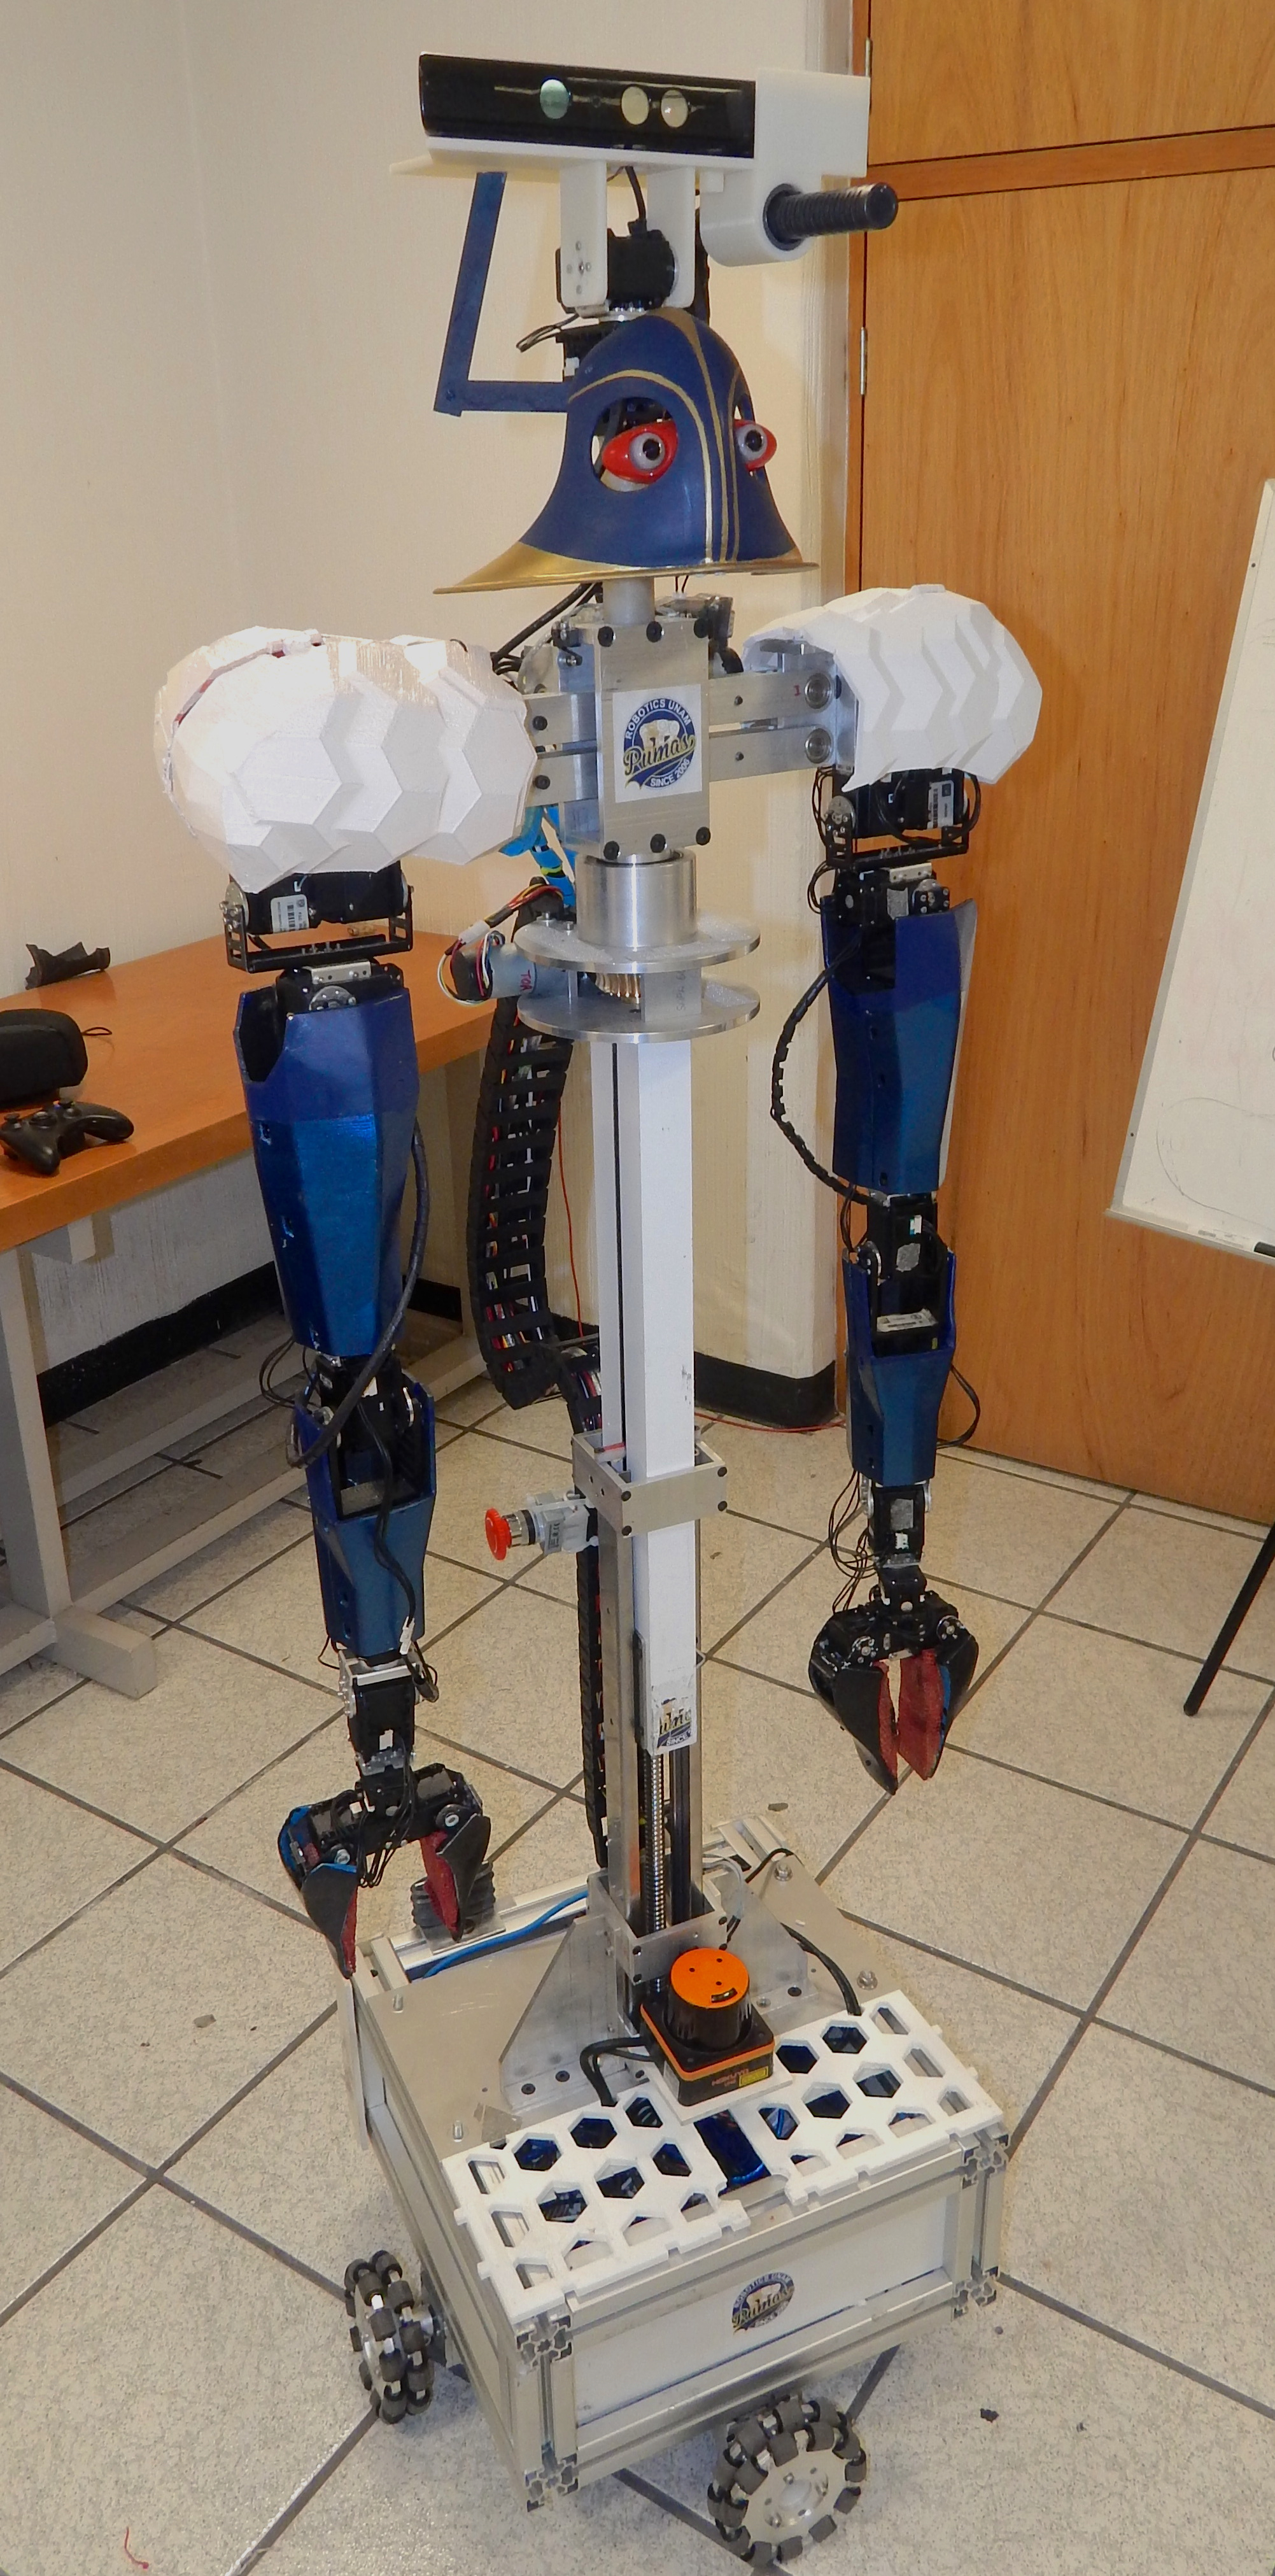
\includegraphics[angle=0, height=11cm, width=6cm\textwidth]{Figures/justina2017.eps}
	%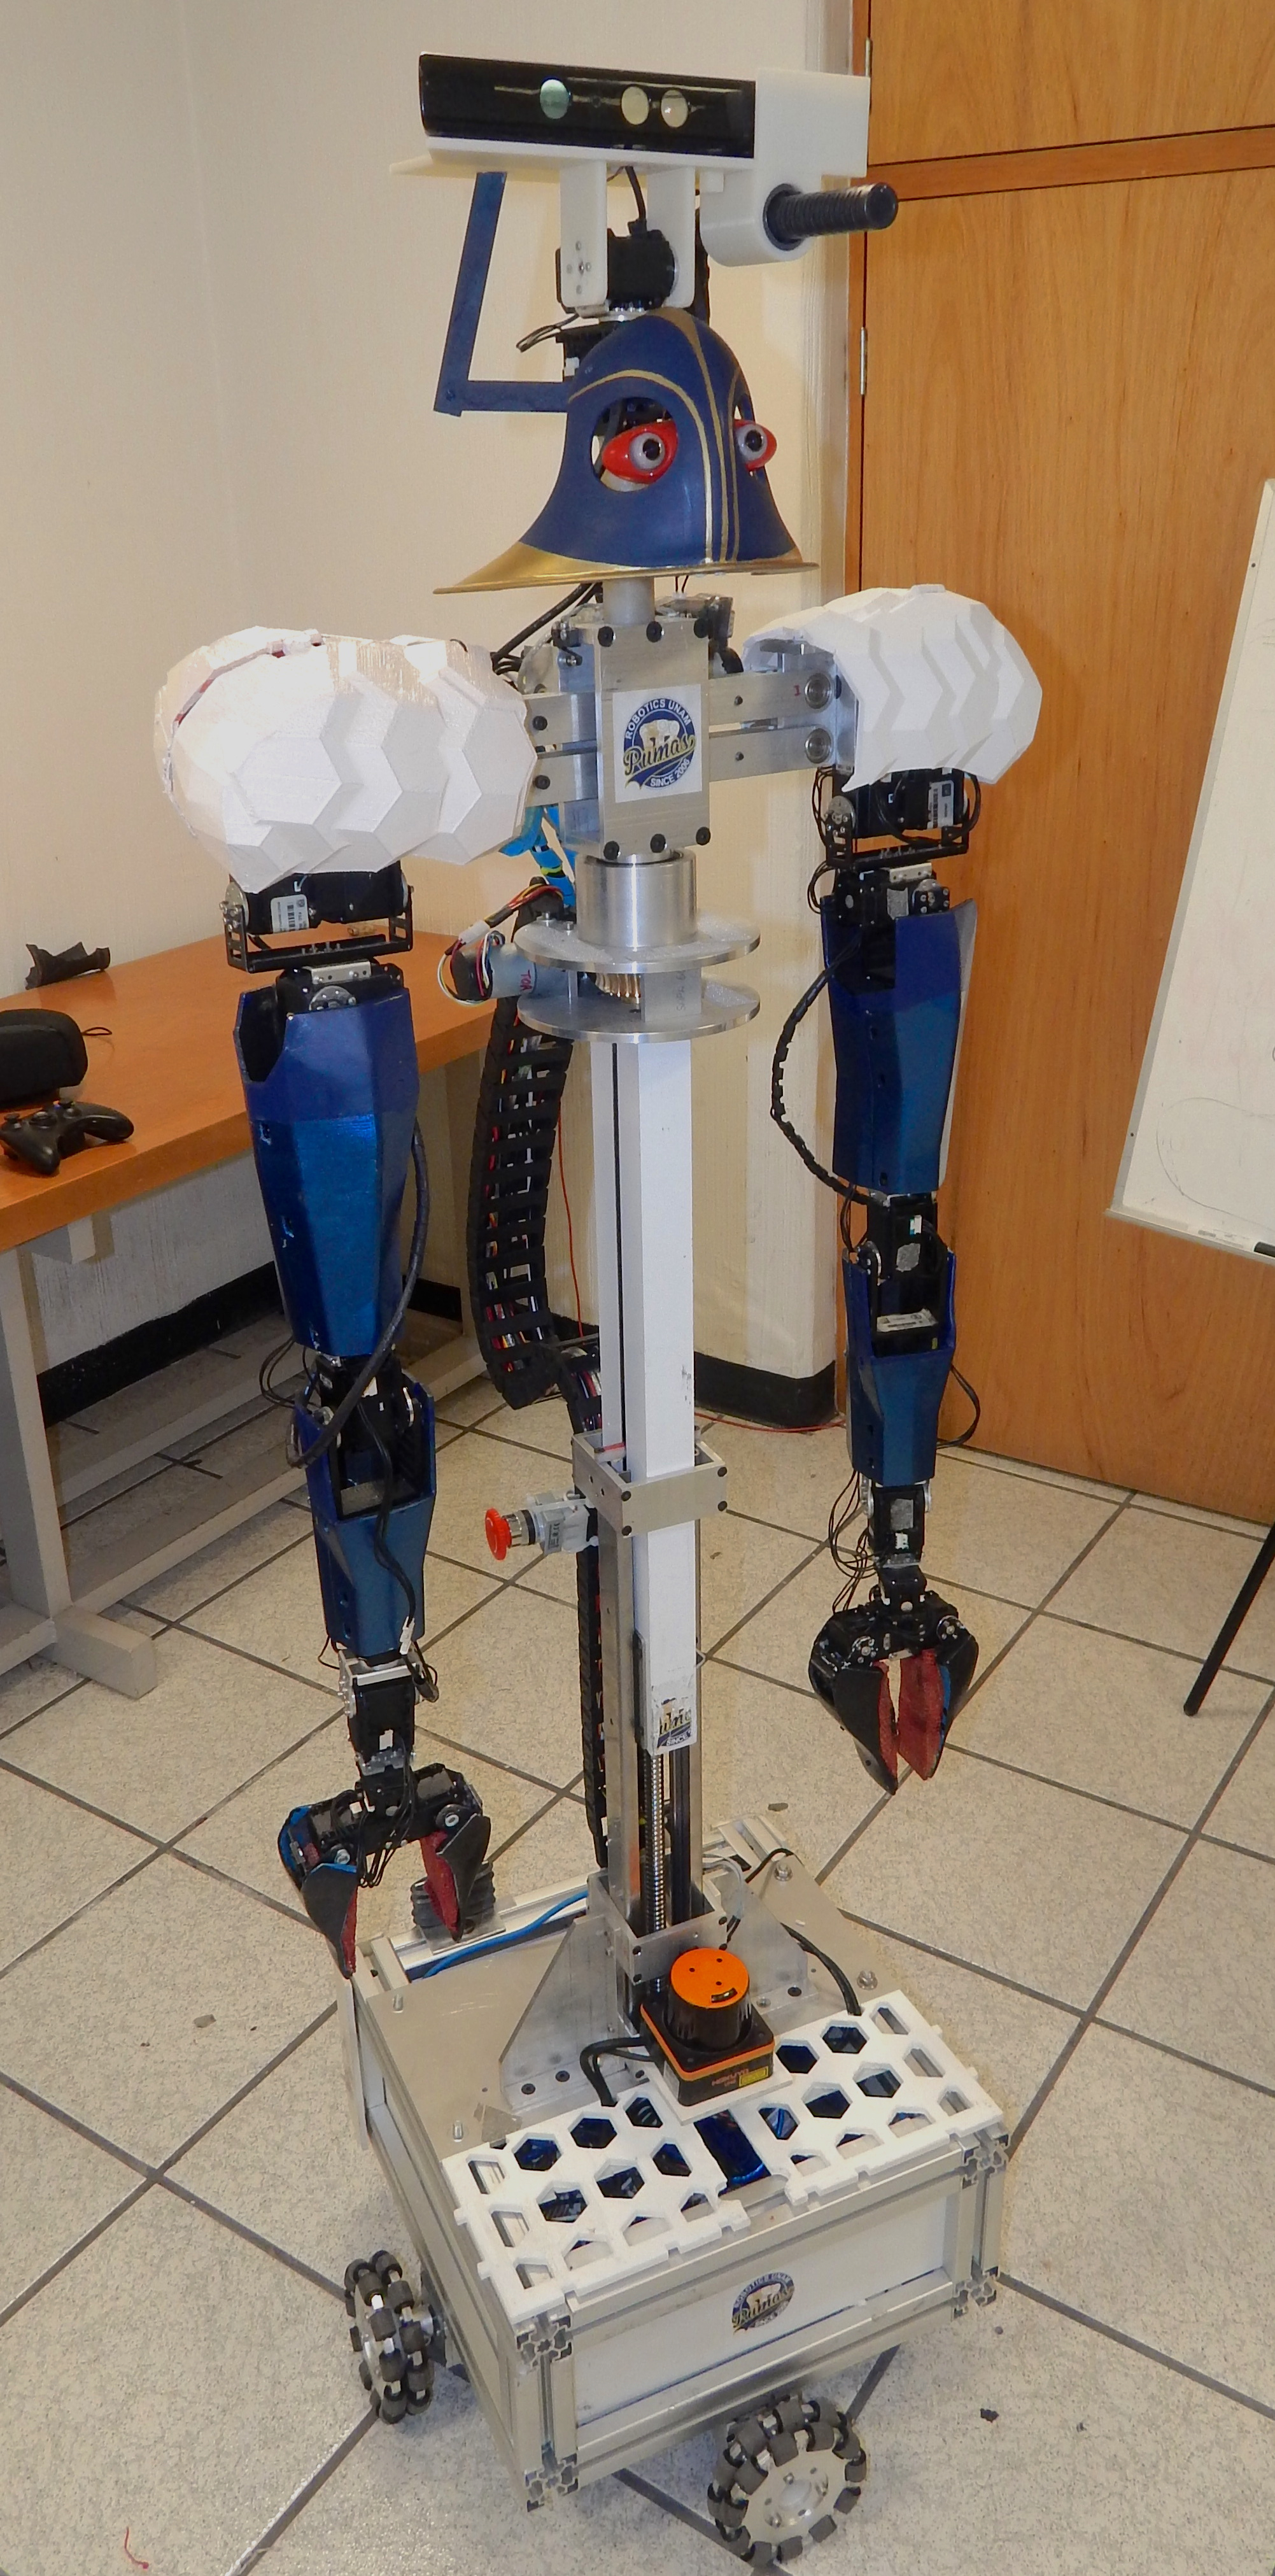
\includegraphics[width=0.48\textwidth]{Figures/justina2017.eps}
  %\end{center}
  \caption{Robot Justina}
  \label{fig:justina}
\end{wrapfigure}



ACTUATORS:

\begin{itemize}
	\item \textbf{Mobile base:} Omnidirectional through differential pair configuration and omnidirectional wheels. 
	\item \textbf{Manipulators:} 2 x 7-DOF anthropomorphic arms with 10 Dynamixel servomotors each.
	\item \textbf{Head:} 2-DOF (Pan and tilt) built with Dynamixel servomotors.
	\item \textbf{Torso:} 1-DOF (Elevation) through a worm screw and a configuration of gears. 
	\item \textbf{Speakers:} Two speakers to generate synthetic speech.
\end{itemize}

SENSORS:

\begin{itemize}
	\item \textbf{RGB-D Camera:} Microsoft's Kinect sensor 
	\item \textbf{RGB Camera:} Logitech Pro C920 Full HD.
	\item \textbf{Microphone:} Rode NTG2 directional microphone.
	\item \textbf{Array of Microphones:} An array of four microphones to detect sound sources.
	\item \textbf{Laser:} Hokuyo rangefinder URG-04LX-UG0.
\end{itemize}

\subsection{Software Configuration}
Our software configuration is based on the VIRBOT architecture \cite{virbot}, 
which provides a platform for the design and development of software for general purpose service robots, see figure \ref{fig:virbot}. 
The VIRBOT architecture is implemented in our robots through several modules that perform well defined tasks \cite{muller}, with a 
high level of interaction between them. The principal framework used for interaction is ROS, where a module is represented by one or 
several ROS's nodes. Also, for modules using the Microsoft operating system, we use our own middleware called Blackboard to
link them with ROS nodes running on Linux.
In the following sections are explained each of the layers of the VIRBOT system.

%\begin{wrapfigure}{R}{0.7\textwidth}
  %%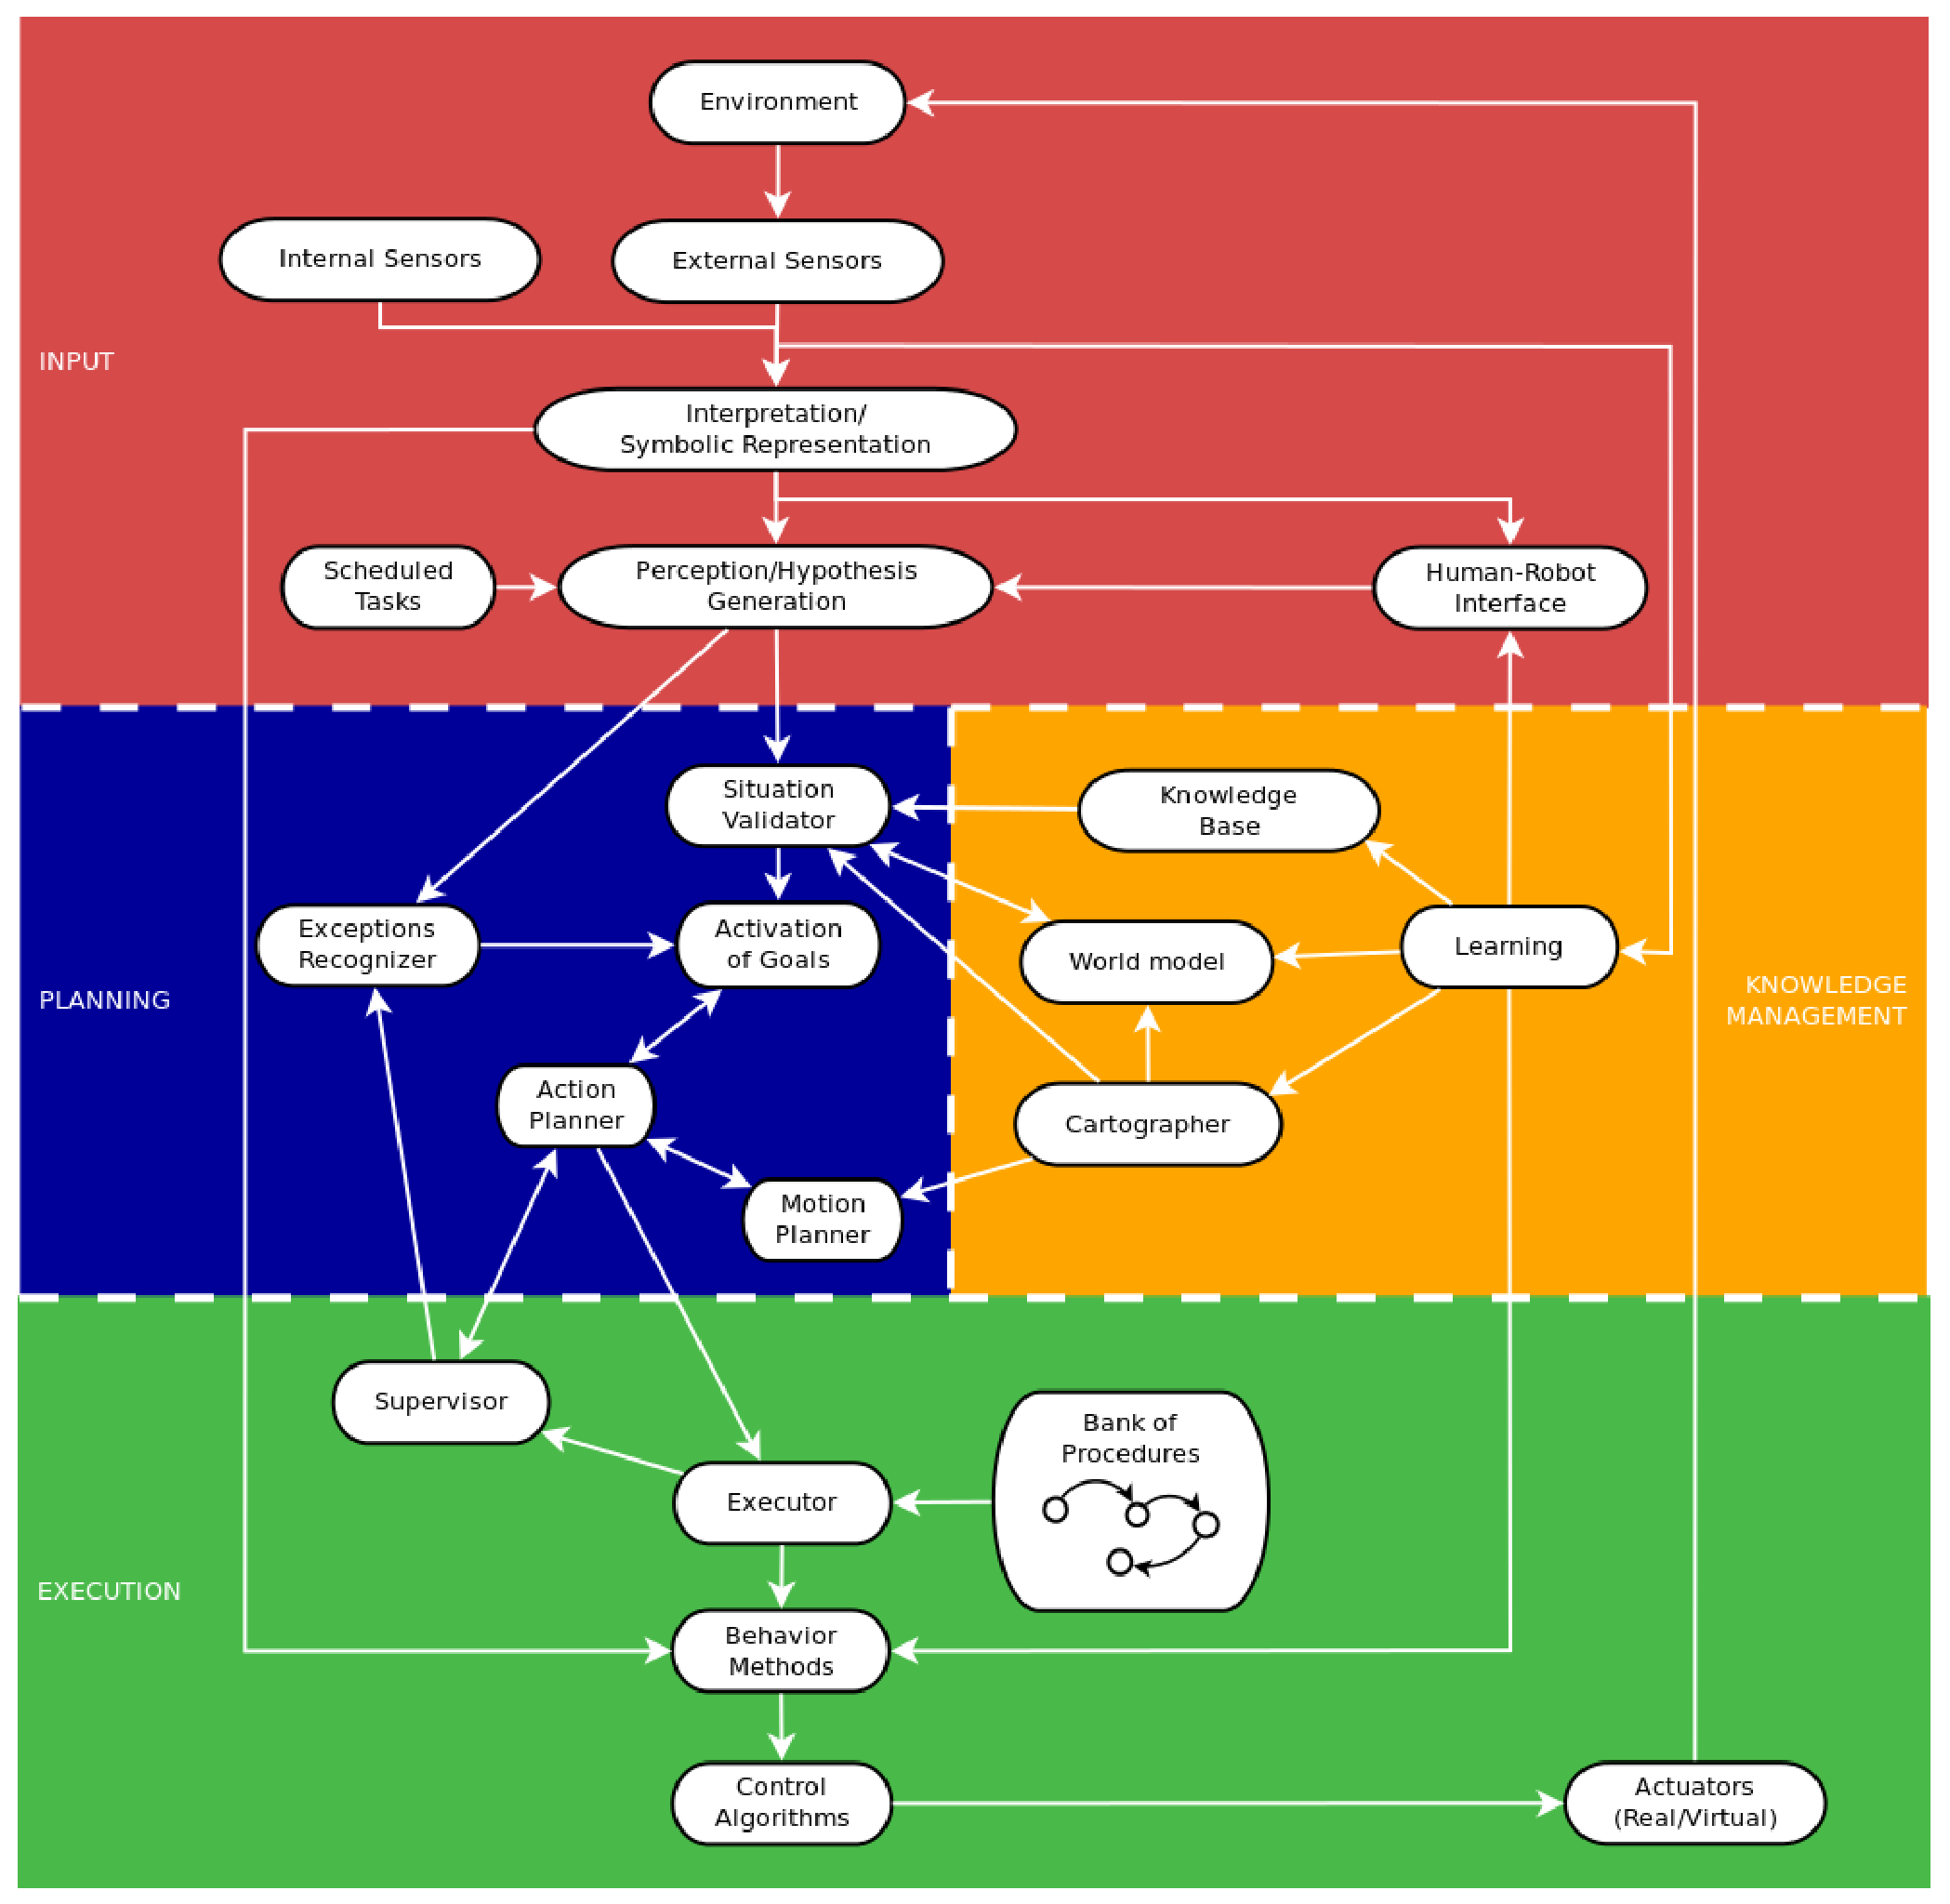
\includegraphics[width=0.48\textwidth]{Figures/ViRBot.eps}
  %%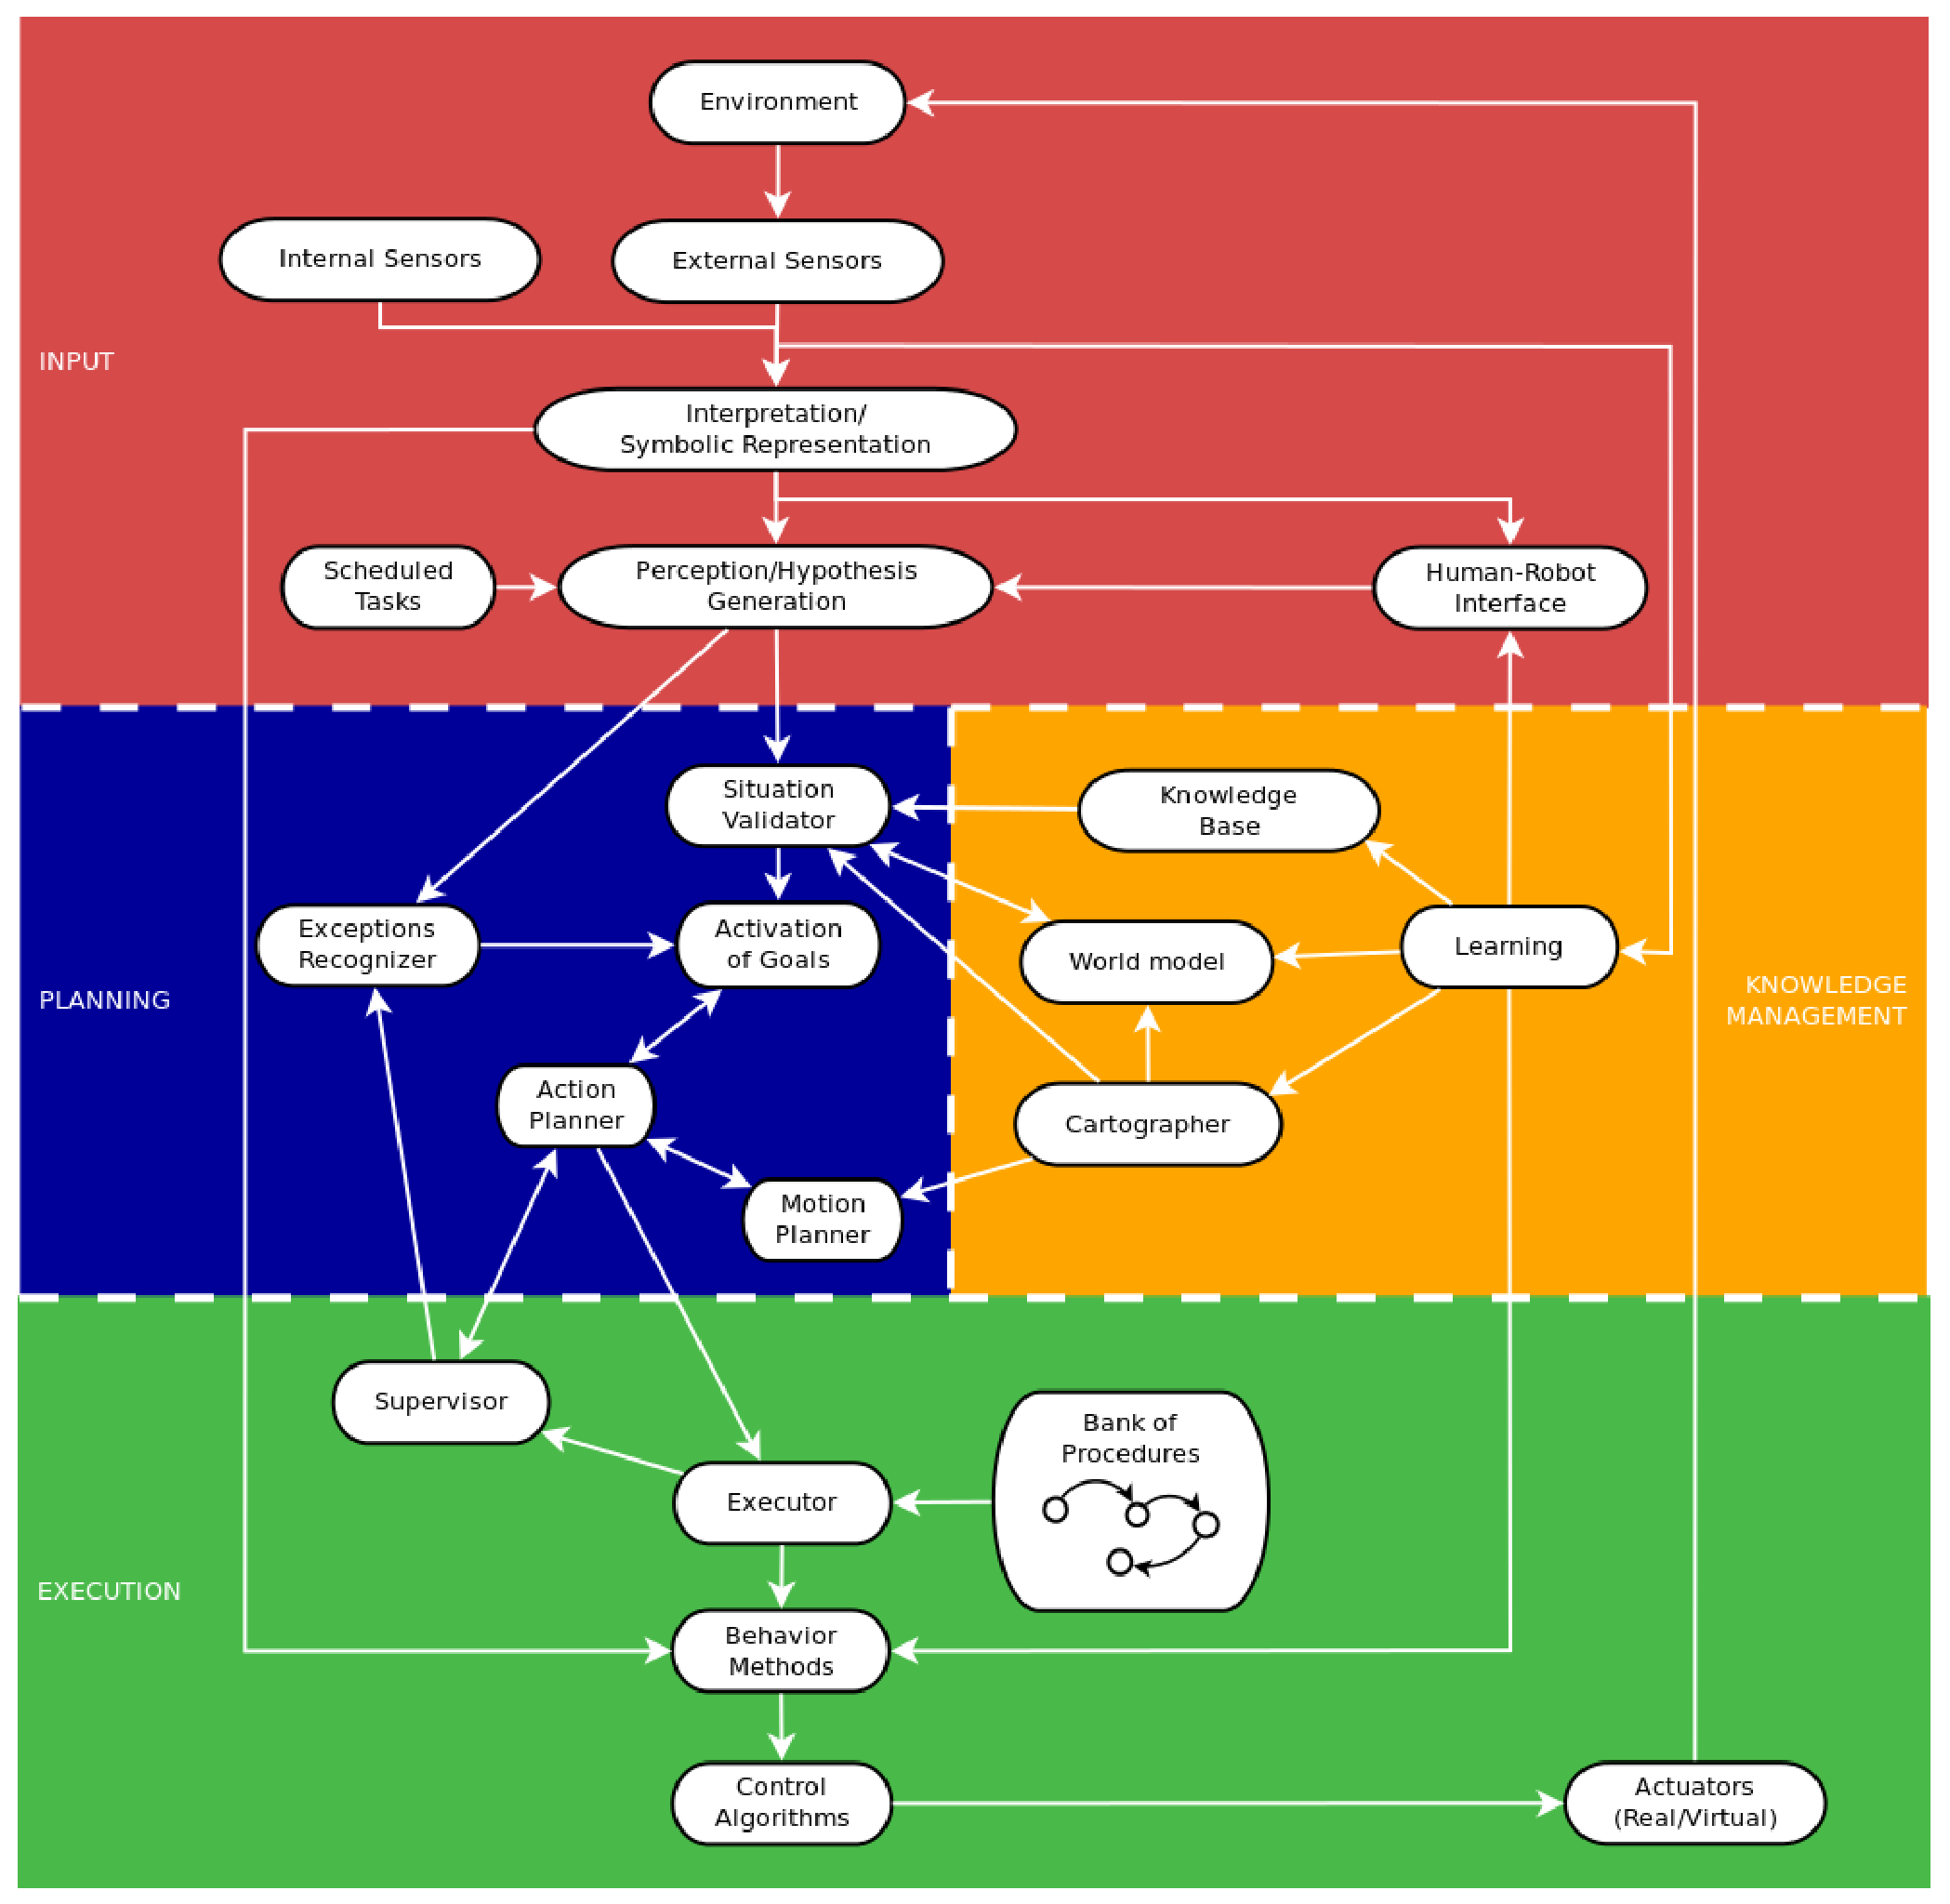
\includegraphics[angle=0, height=13cm, width=9cm]{Figures/ViRBot.eps}
  %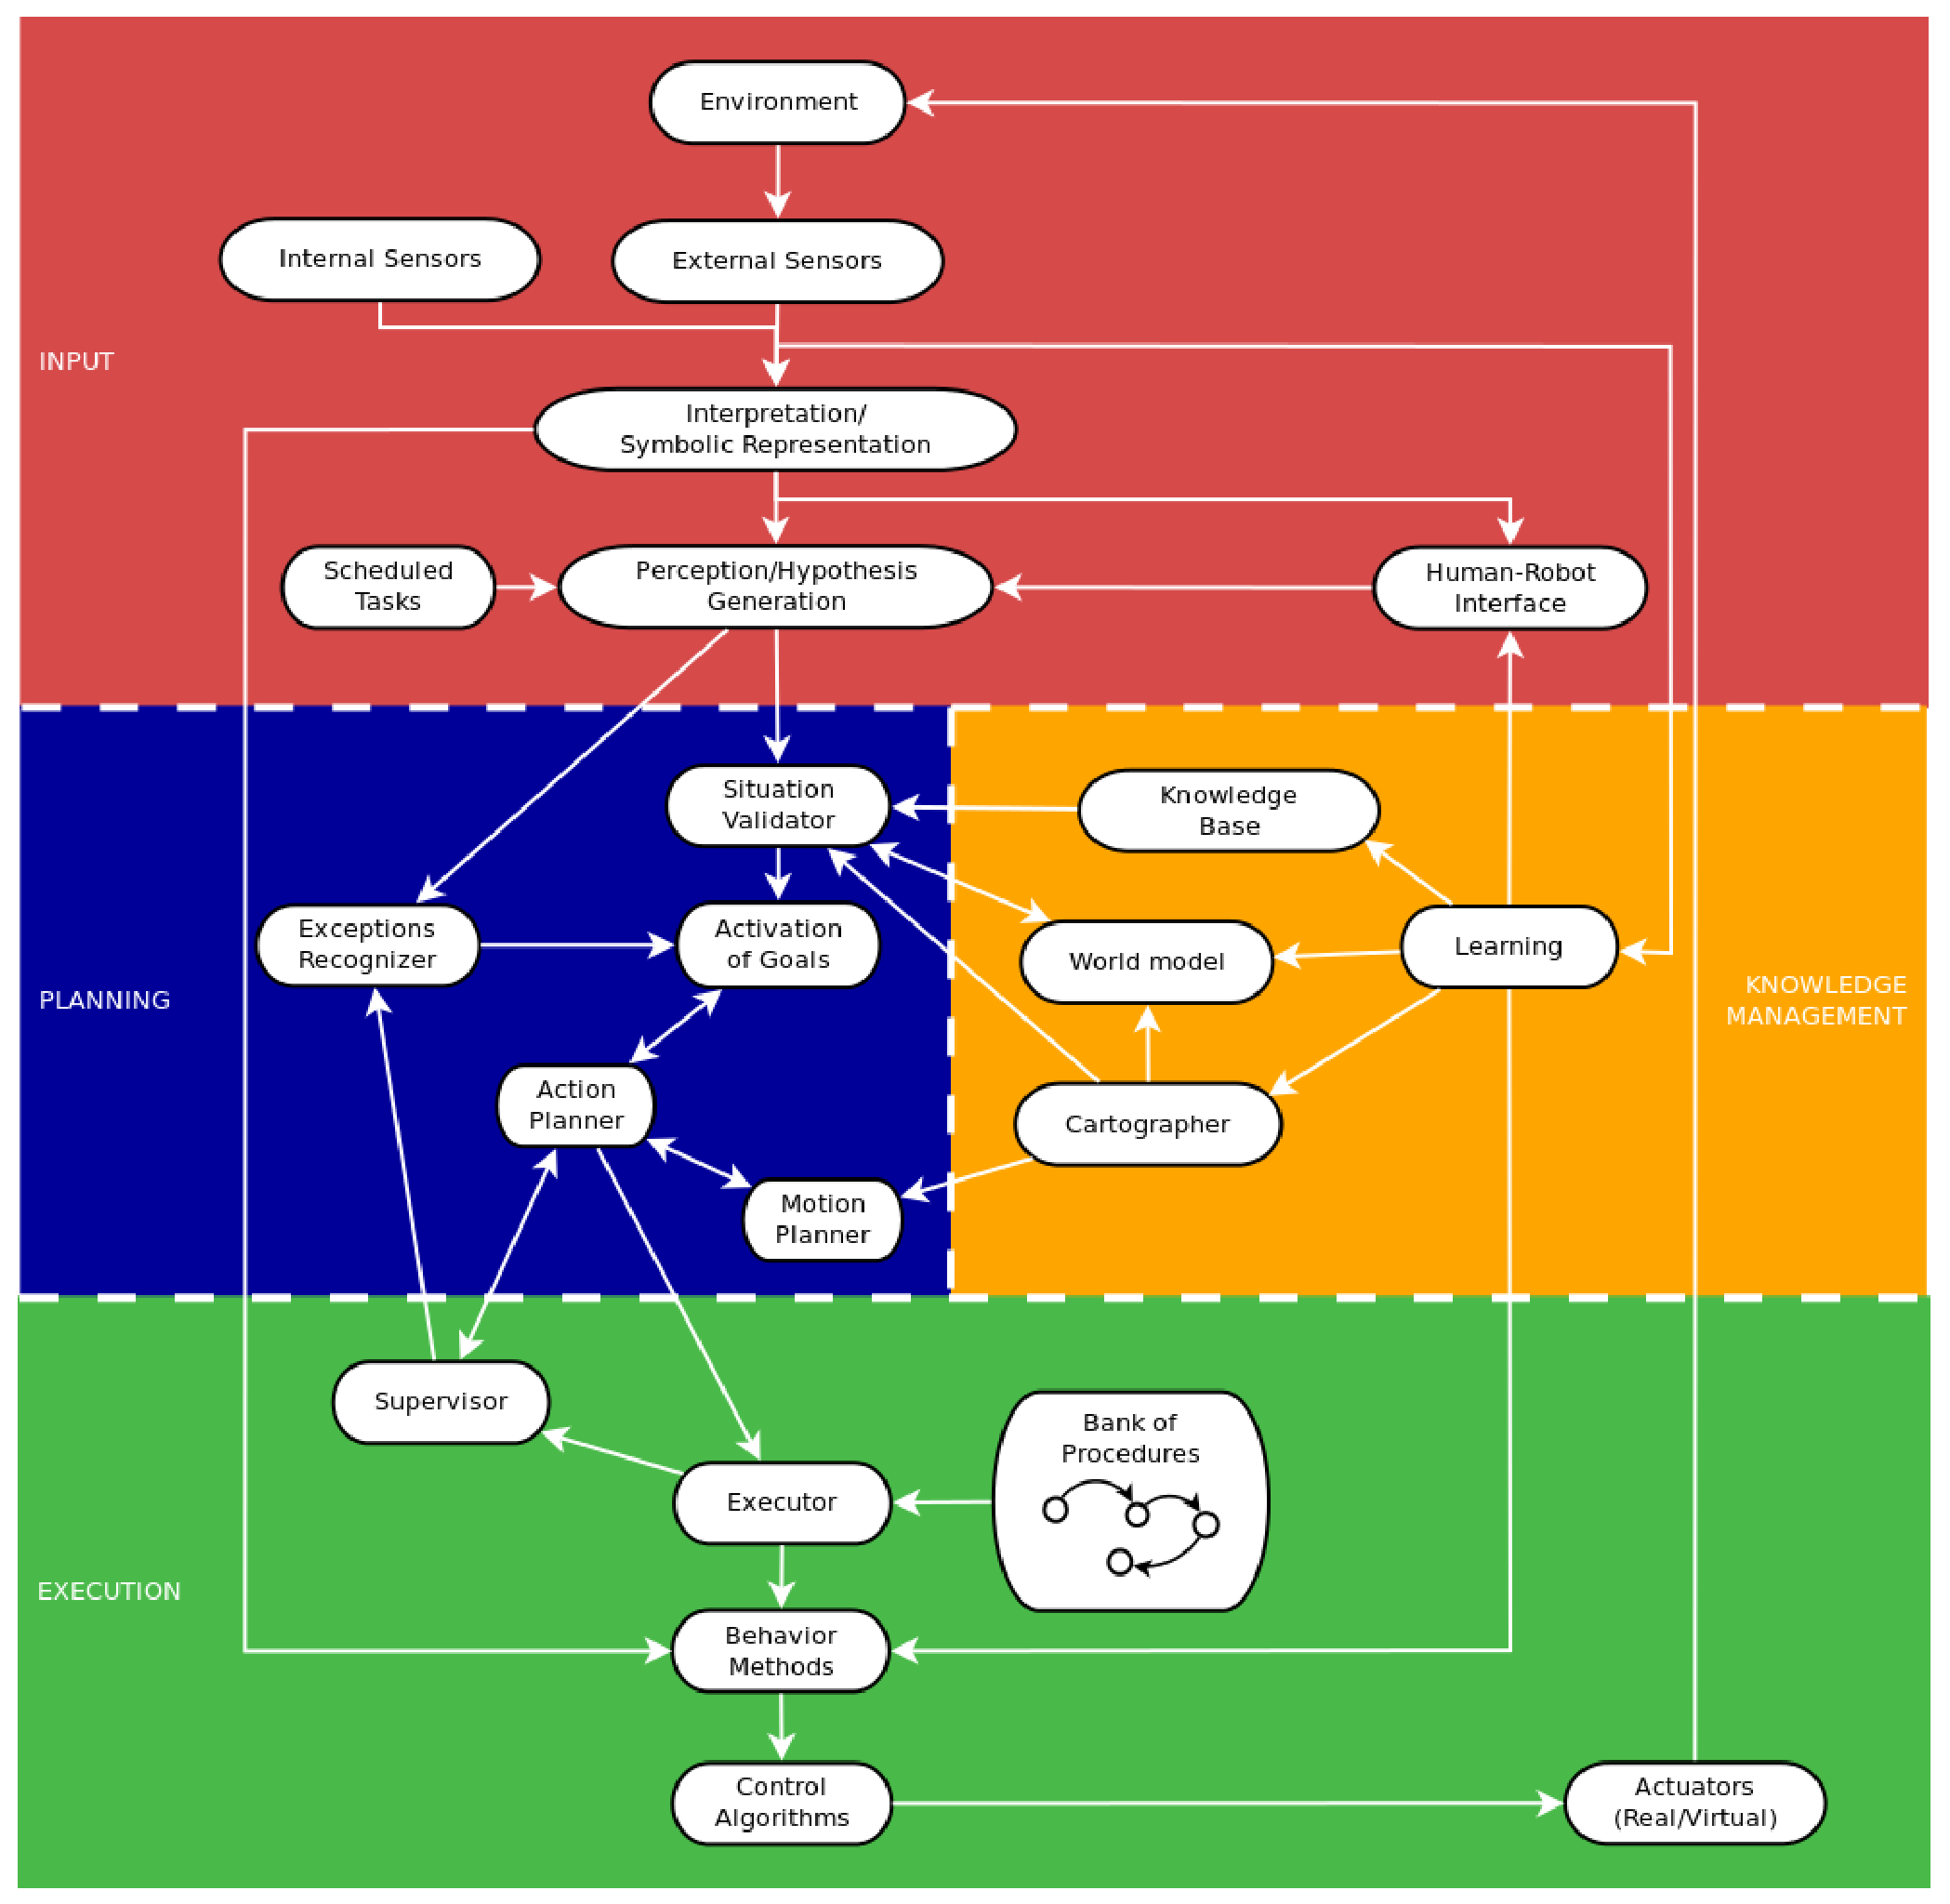
\includegraphics[angle=0, height=14cm, width=12cm]{Figures/ViRBot.eps}
  %\caption{Block diagram of the ViRBot architecture.}
  %\label{fig:virbot}
%\end{wrapfigure}




\begin{figure}[h]
	\centering
	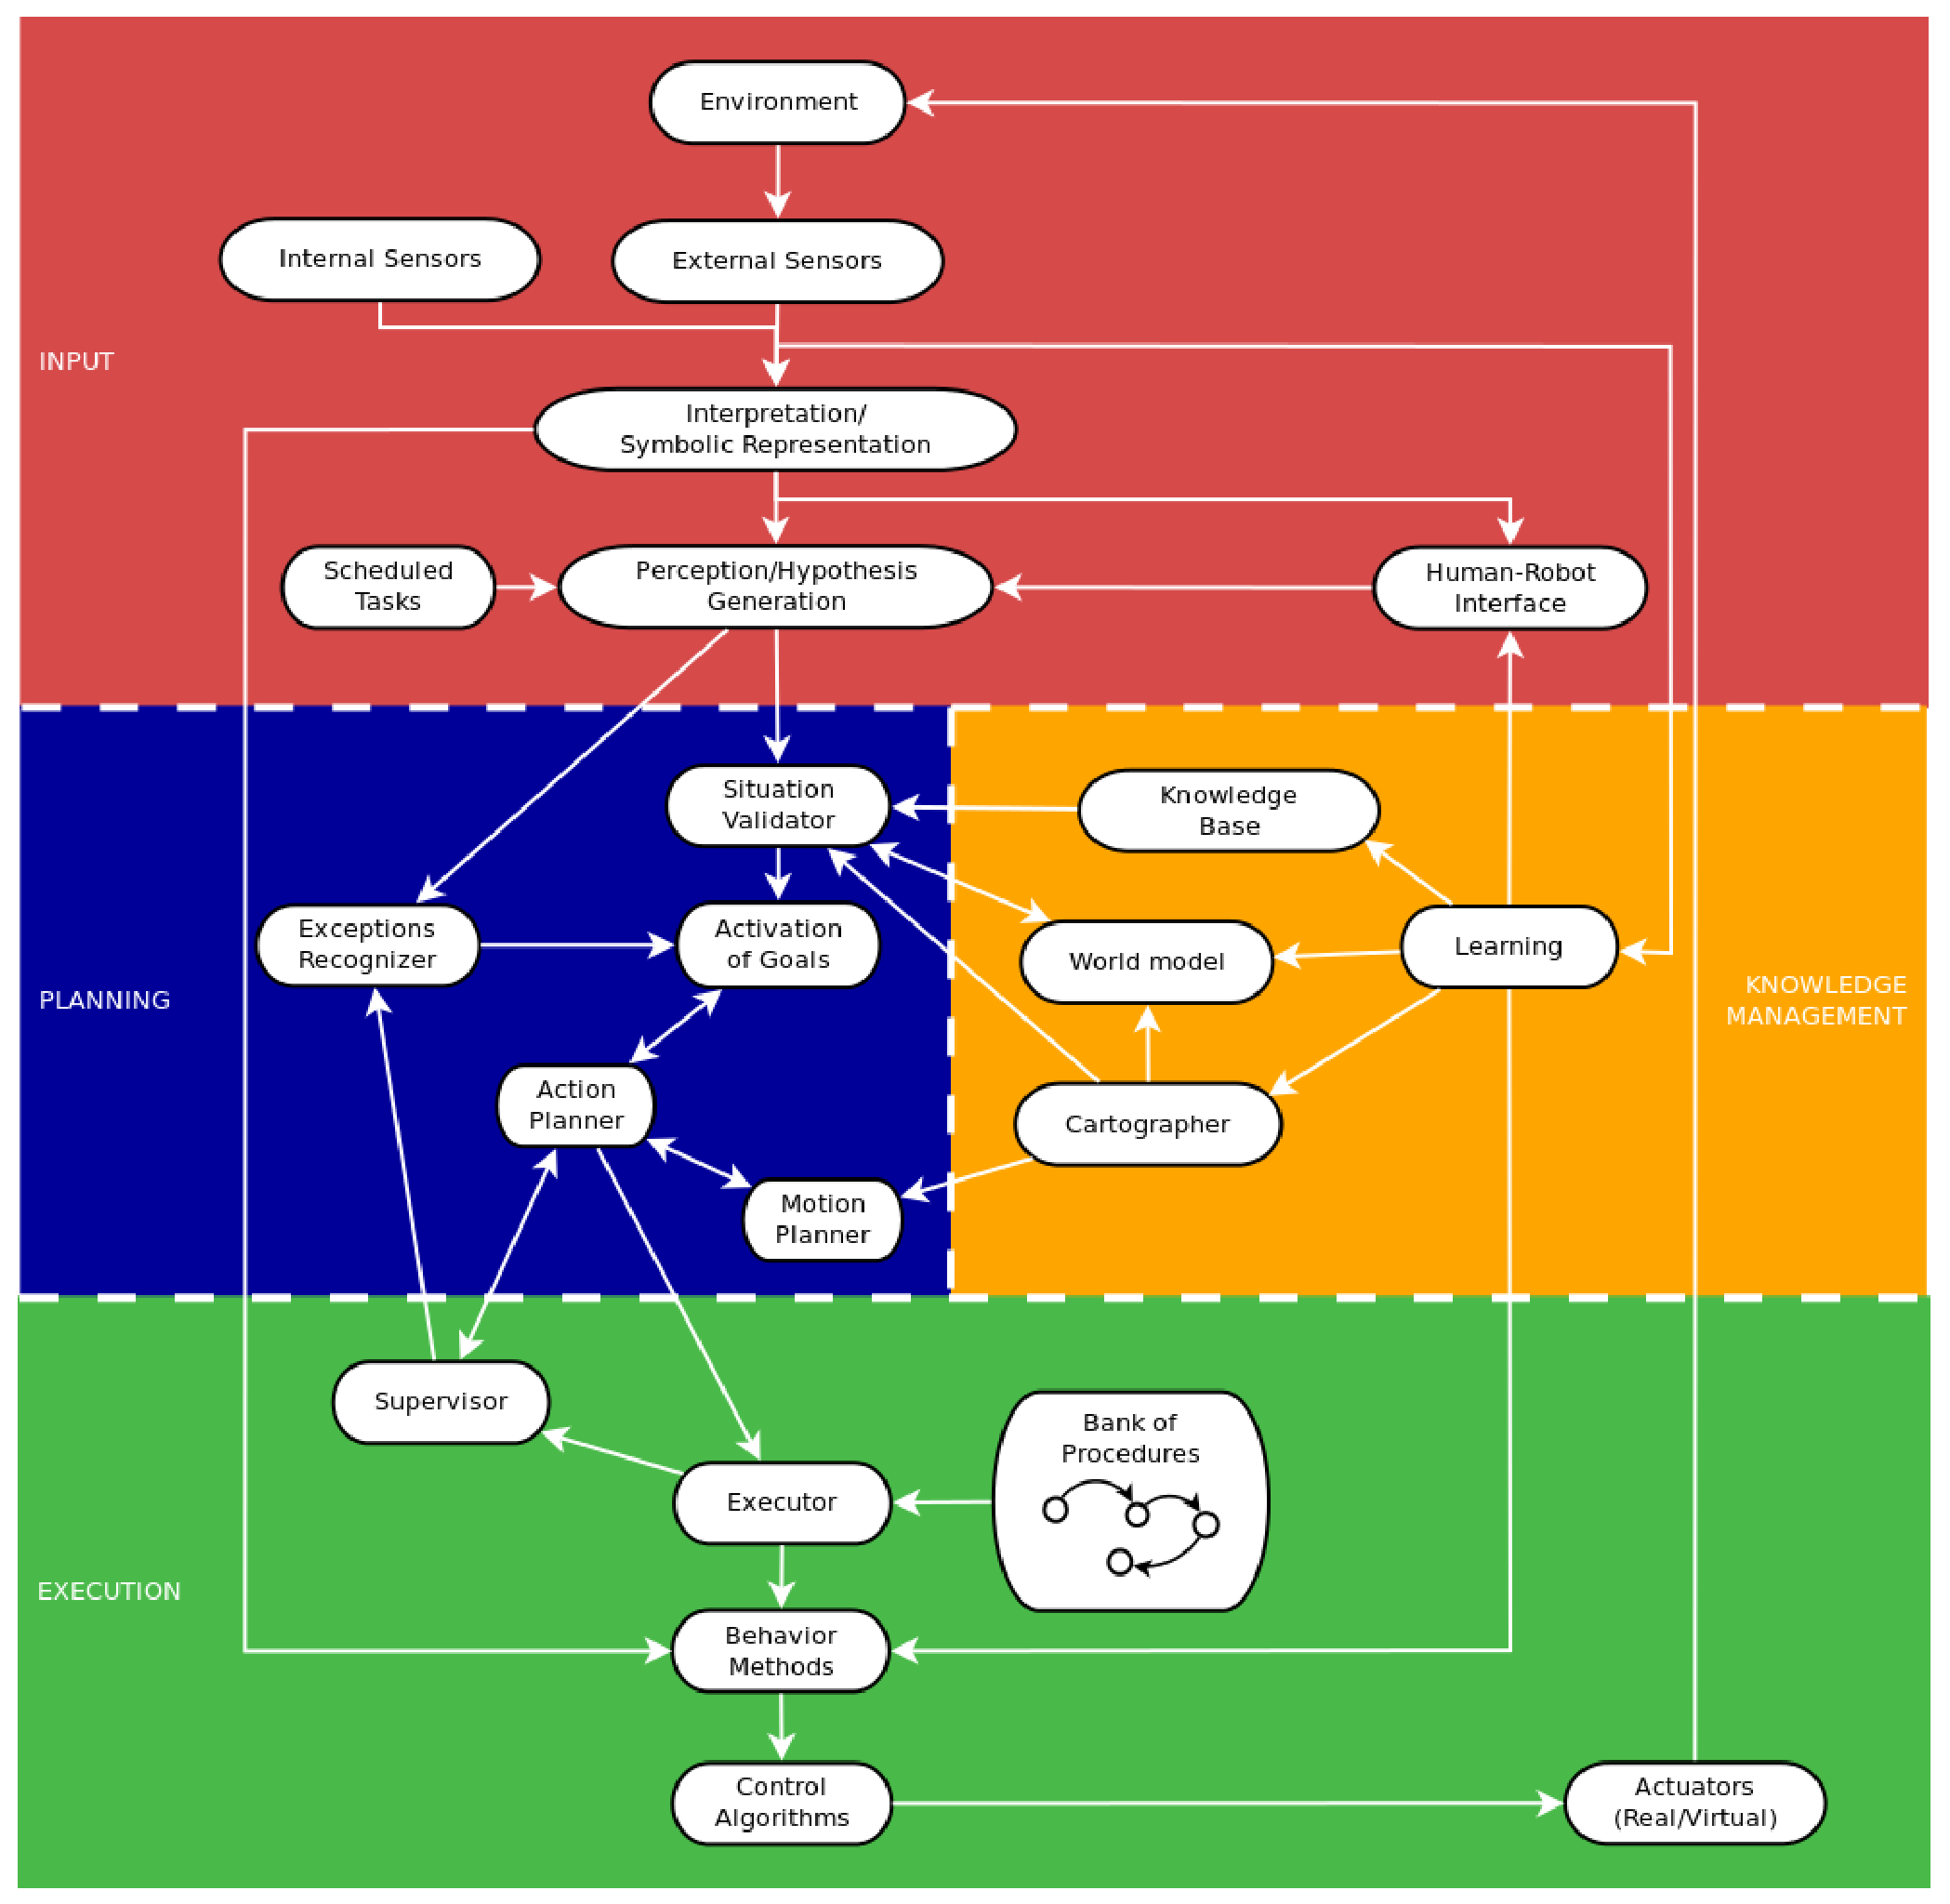
\includegraphics[angle=0, height=12cm, width=12cm]{Figures/ViRBot.eps}
	\caption{Block diagram of the ViRBot architecture.}
	\label{fig:virbot}
\end{figure}

%\newpage

\subsection{Inputs Layer}

This layer process the data from the robot's internal and external sensors, 
they provide information of the internal state of the robot, as well as, the external world where the robot interacts.
In some of Justina's designs it has lasers, sonars, infrared, microphones and stereo and RGB-D cameras.
Digital signal processing techniques are applied to the data provided by the internal and external sensors to
obtain a symbolic representation of the data, as well as, to recognize and to process voice and visual data.
Pattern recognition techniques are used to create models of the objects and the persons that interact with the robot.
With the symbolic representation this module generates a series of beliefs, that represent the state of the environment where
the robot interacts.


\subsection{Planning Layer}

The beliefs generated by the perception module are validated by this layer, it uses the Knowledge Management layer
to validate them, thus a situation recognition is created.
Given a situation recognition, a set of goals are activated to solve it.
Action planning finds a sequence of physical operations to achieve the activated goals.


\subsection{Knowledge Management Layer}

This layer has different types of maps for the representation of the environment, they are created using 
SLAM techniques.
Also in this layer there is a localization system, that uses the Kalman filter, to estimate the robot's position and orientation.
A rule based system, CLIPS, developed by NASA, is used to represent the robot's knowledge, in which each rule contains the
encoded knowledge of an expert.


\subsection{Execution Layer}
This layer executes the actions and movements plans and it checks that they are executed accordingly.
A set of hardwired procedures, represented by state machines, are used to partially solve specific problems, finding persons,
object manipulation, etc. The action planner uses these bank of procedures and it joins some of them to generate a plan.


%%%%%%%%%%%%%%%%%%%
%%% CURRENT RESEARCH  %%%
%%%%%%%%%%%%%%%%%%%

\section{Current research}\label{sec:CurrentResearch}
In this section is presented the current research developed in our laboratory to improve the performance of our service
robots.

\subsection{RGB-D representation of the environments}\label{subsec:SurfRecon}
For the construction of roadmaps, 3D data is used to find the occupied and free space where a robot can
navigate, it uses clustering techniques to find a representation of them.
The free space is found by separating the objects' and walls' planes from the floor's plane, that represents the space where the mobile
robot navigates.
The RGB-D cameras provide information through a cloud of points that represent the spatial position of each pixel of the 
captured image.  In this research, the RGB information provided by the camera is not used, for the
robot only collects 3D readings, \(R=\{ r_1,r_2,...,r_{N}\}\),
\(r_j = (x_{screen_j},y_{screen_j},d_j)\) , where \(x_{screen_j},y_{screen_j}\) represent the pixel location in the captured image and
\(d_j\) the distance to the objects in line of sight.
Then \(q_j = (x_j,y_j,z_j)\), represents the spatial positions of the objects' points relative to the Kinect's position, mounted
in top of the robot's mechatronic head.

The number of points captured by a 3D sensor in just one picture is immense, around 300,000 points, thus, it is necessary to 
compress the 3D data to a minimum, to be able to find a proper representation of them. For this, clustering techniques are used,
vector quantization (VQ), which also they help to partition the free space into regions, and the centroids of the regions become
the nodes of a roadmap, that is used by a mobile robot to navigate.


 Given a set of \(N_v\) vectors, \(q_j=\{x_j,y_j,z_j\}; j=1,...,N_v\) that represent the position of the cloud points a set of
centroids which represents these vectors is found.
A collection of centroids is called a codebook.  The codebook is designed from a long training sequence that is representative of all
vectors \(q_j\) to be encoded by the system.
A modified VQ algorithm for 3D \cite{Marco} data is as follows:

\vspace{0.1 in}

 \begin{itemize}[nolistsep,noitemsep]
\item 1. Find an initial codebook \(D_1\), with one centroid \(C_1\), by averaging all the vectors \(q_j\), with \(L=1\) and \(m=1\).

%\vspace{0.1 in}
\item 2. Modify each of the centroids \(C_i;i=1,...,L_m\) in \(D_m\) by adding them a vector \(\pm\psi\)
of small magnitude to generate 2 new centroids from each of them, generating a new codebook  \(D_{m+1} \), and
\( L_{m+1} = 2*L_m \), \(m=m+1\).

%\vspace{0.1 in}
\item 3. Given a codebook \(D_m={C_i;i=1,...,L_m}\) assign each vector \(q_j\) into the
clusters \(R_k\) whose centroid \(C_k\) is closer to \(q_j\) according to some
similitude measurement \(d_j = d(q_j,C_k)\). The measurement used is the Euclidean distance between two points.

%\vspace{0.1 in}
\item 4. Recompute the centroids \(C_k\) for each of the clusters, \(R_k\), by averaging all the vectors
\(q_j\) that belong to \(R_k\).

%\vspace{0.1 in}
\item 5. If the difference between the average distance \(\bar d_t = \frac {1} {N_v} \Sigma d(q_j,C_k)\), in iteration \(t\), between vectors \(q_j\)
and their corresponding centroids \(C_k\), and the previous average distance \(\bar d_{t-1} \), \(| \bar d_t - \bar d_{t-1} | \ge \epsilon\),
go to 3.

%\vspace{0.1 in}
\item 6. If \(L_m <\)  codebook size go to 2.
\end{itemize}


\vspace{0.1 in}

 Where codebook size is the number of regions of the environment.
Figure \ref{fig:ResultingClusters} shows in the left side the original RGB image captured by the Kinect, in the center
it is shown the free space clusters in green and the occupied space clusters, in purple, the black regions are those points with no 
depth information. In the right it is shown the resulting environment representation. Green dots represent the nodes,
free space centroids, used to build the roadmap and calculate a path. Purple rectangles represent obstacles and the red lines are 
the path calculated by Dijkstra algorithm to reach the goal point, also colored in red.


\begin{figure}[!ht]
\begin{center}
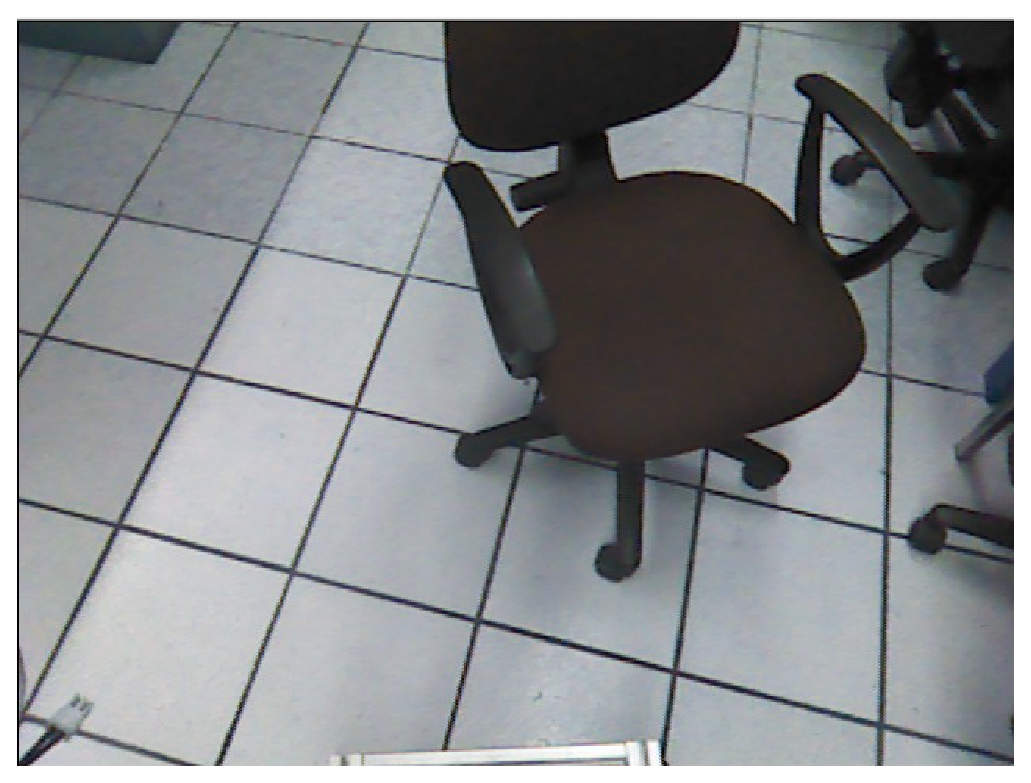
\includegraphics[width=3.65cm,width=3.0cm]{Figures/VQ_Original.eps}
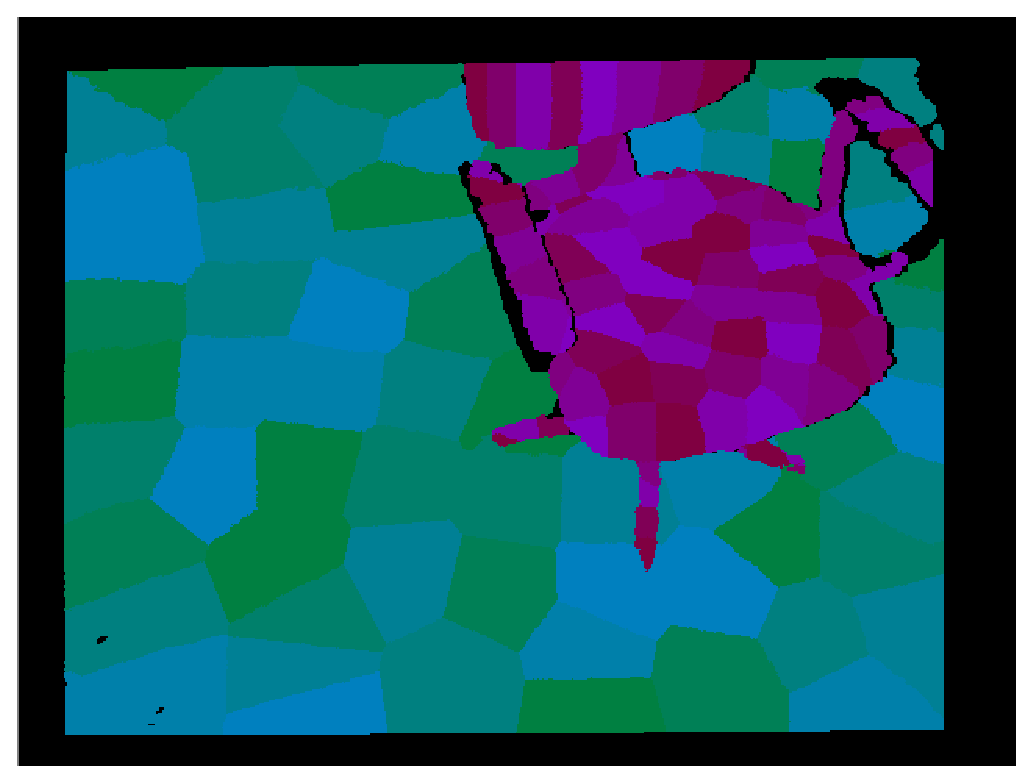
\includegraphics[width=3.65cm,width=3.0cm]{Figures/VQ_Clustered.eps}
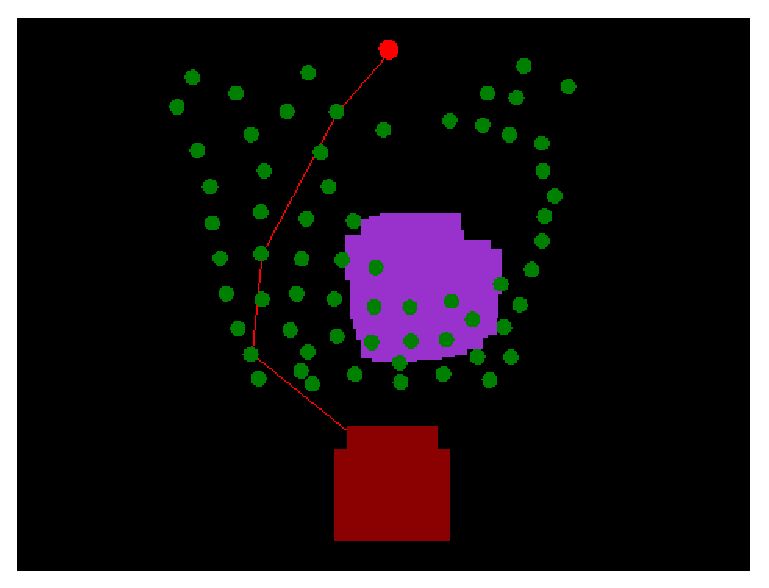
\includegraphics[width=3.65cm,width=3.0cm]{Figures/VQ_Map.eps}
\end{center}
\caption{\textbf{Left:} Original RGB image captured by the Kinect. \textbf{Center:} Free space clusters and occupied space clusters.
\textbf{Right:} Resulting environment representation.}
\label{fig:ResultingClusters}
\end{figure}

To obtain real time performance the VQ algorithm was processed in parallel in a GPU programmed with CUDA, it was also implemented
the whole process sequentially, using C++, to compare processing times and to test the effectiveness of the parallel 
implementation. Table \ref{tab:Times} shows the results obtained comparing the VQ implementation in parallel and in sequentially of 
the environment's 3D data.
As we can see for the results shown in this table, the parallel implementation of the VQ algorithm is in average 17 times faster 
than the sequentially one, thus this technique can be used by the robot in real time when it navigates.


\begin{table}
\centering
\begin{tabular}{|l|l|}
\hline
Sequential Time [s] & Parallel Time [s]\\
\hline
$\qquad$1.341 & $\qquad$0.078\\
$\qquad$1.373 & $\qquad$0.078\\
$\qquad$1.341 & $\qquad$0.078\\
$\qquad$1.388 & $\qquad$0.077\\
%$\qquad$1.404 & $\qquad$0.078\\
$\qquad$1.357 & $\qquad$0.078\\
\hline
\end{tabular}
\caption{Comparison of processing time for serial and parallel implementations of the VQ algorithm.}
\label{tab:Times}
\end{table}



%To align several captures of point clouds of a scene, an implementation of the ICP 
%(Iterative Closest Point) algorithm is used. Also, a reduction of data is implemented using Vector Quantization 
%\cite{linde1980algorithm}. 
%The virtual environment builded can ve visualised using the simulator described in subsection
%\ref{subsec:Simulator}. 

%The system was successfully tested experimentally by reconstructing part of the environment in the @Home arena in the
%2016 RoboCup in Leipzig, Germany. Figure \ref{fig:SurfRecon} shows an image of multiple point clouds sets captured by the robot 
%and the virtual environment created.

%\begin{figure}
	%\centering
	%\begin{subfigure}{0.49\textwidth}
		%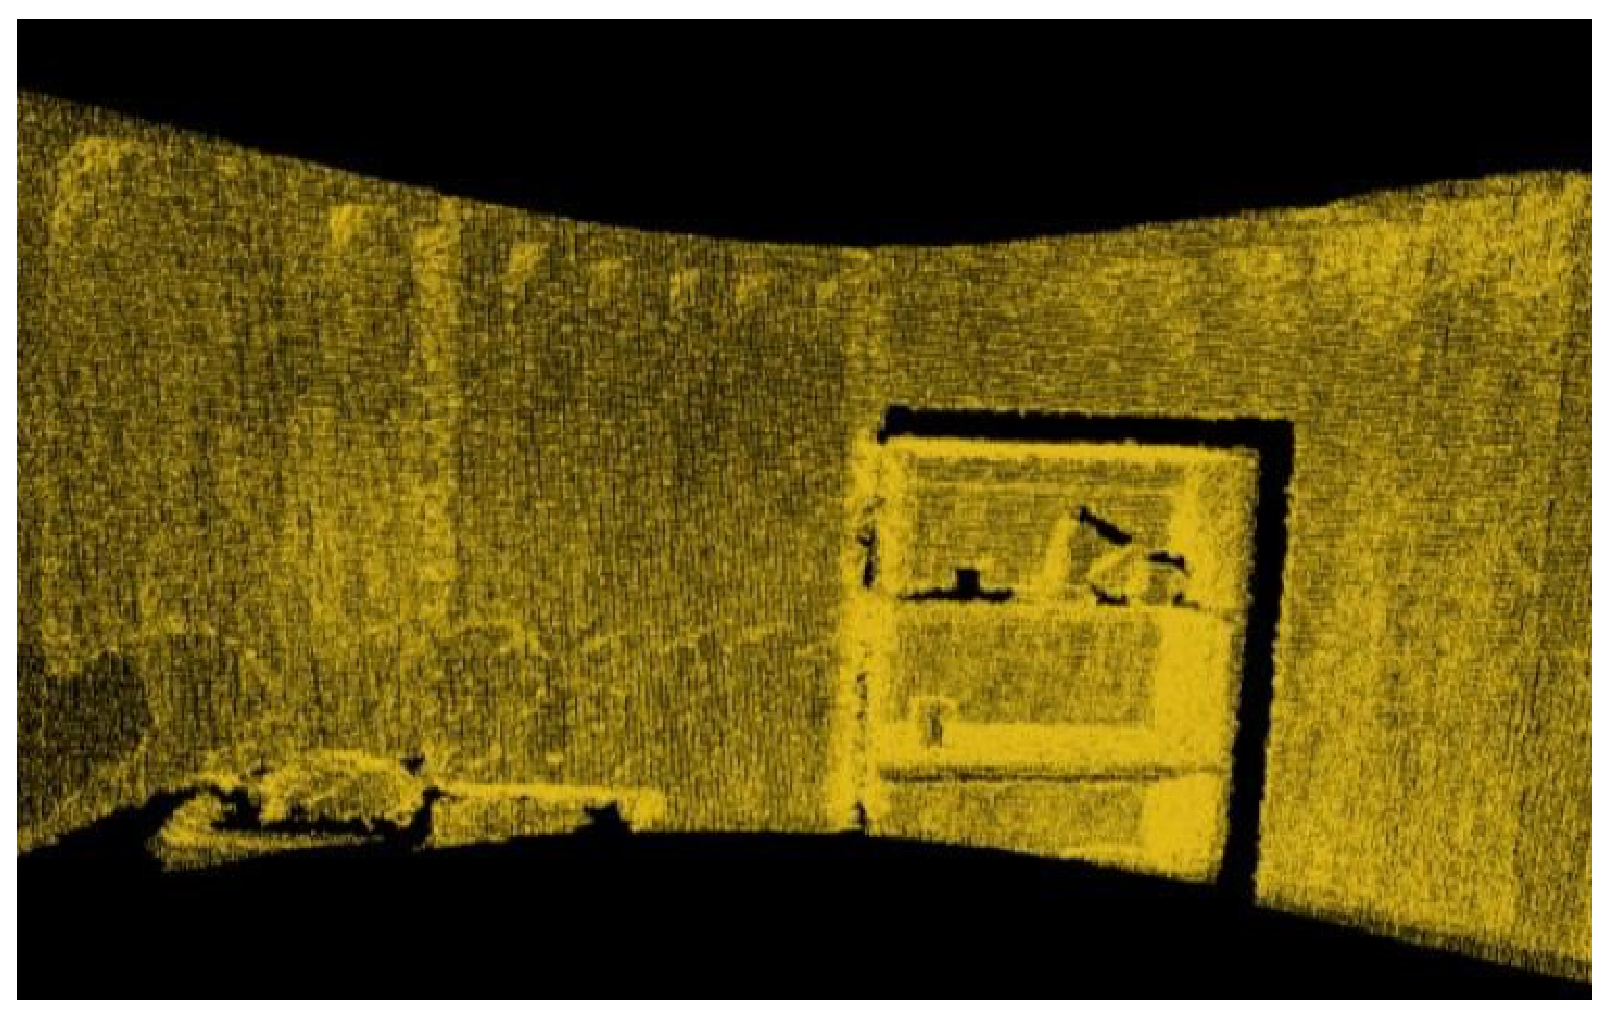
\includegraphics[width=\textwidth]{Figures/envReco1.eps} 
		%\caption{ Several point clouds captures of a scene.}
		%\label{fig:SurfRecon1}
	%\end{subfigure}
	%\begin{subfigure}{0.49\textwidth}
		%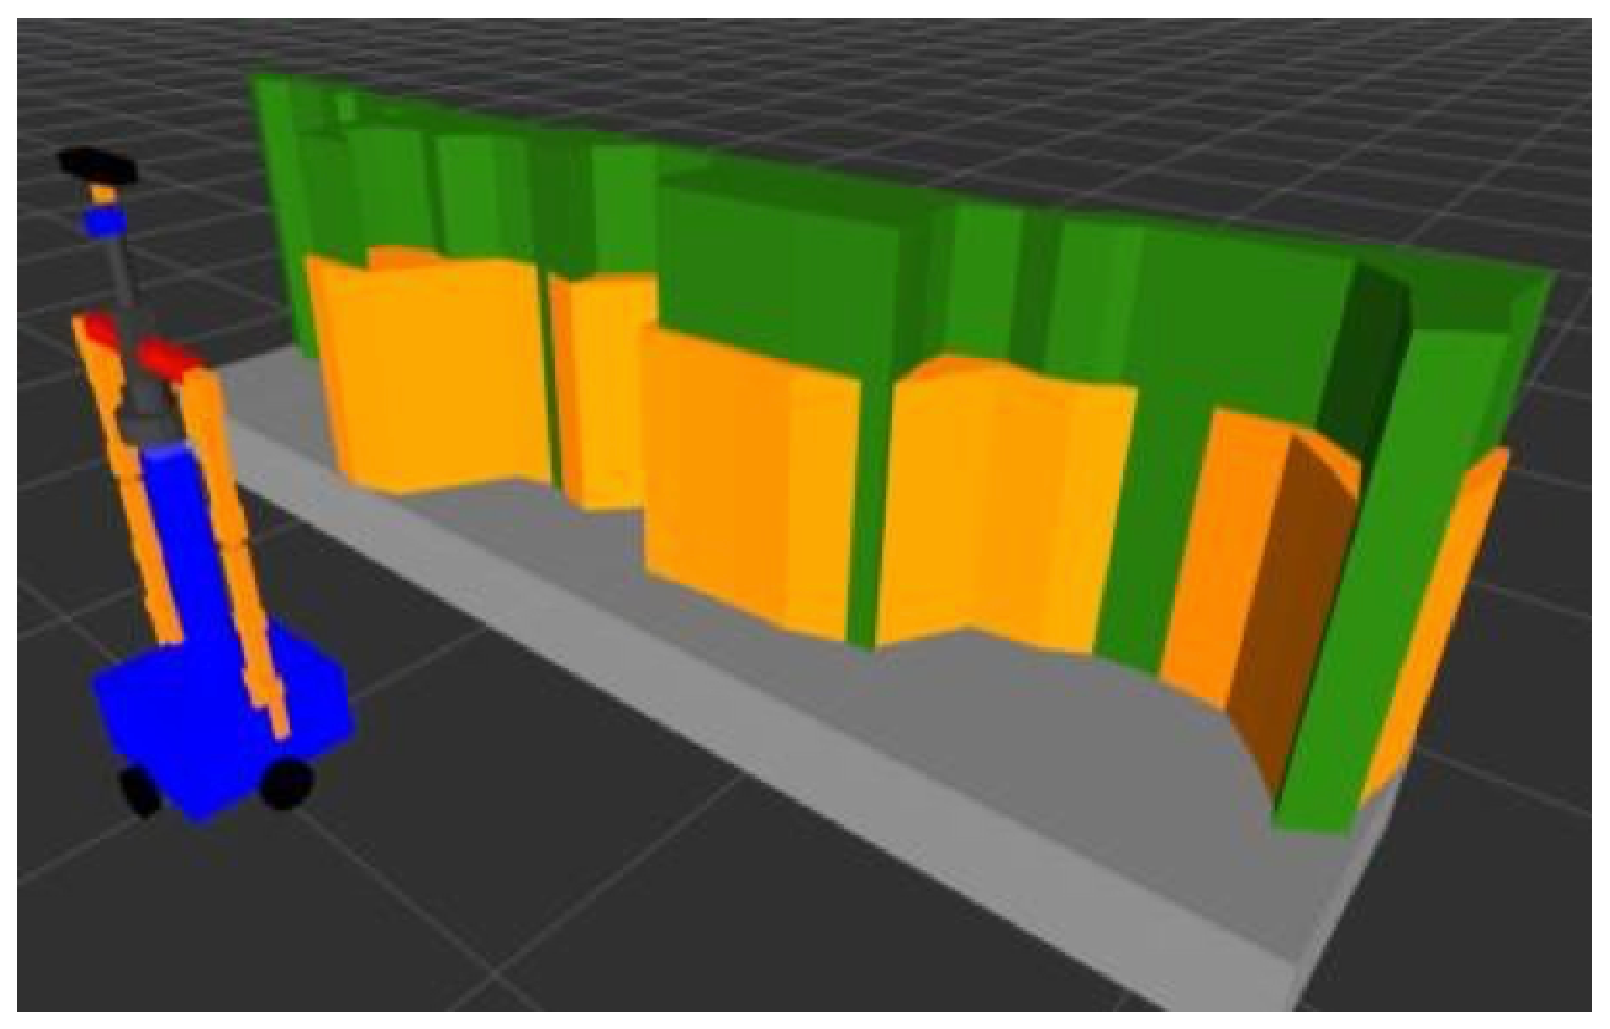
\includegraphics[width=\textwidth]{Figures/envReco2.eps}
		%\caption{Virtual environment build after processing the sets.}
		%\label{fig:SurfRecon2}
	%\end{subfigure}
	%\caption{Example of the test performed in a real scene.}
	%\label{fig:SurfRecon}
%\end{figure}


%\subsection{Service Mobile Robot Simulator}\label{subsec:Simulator}

%Despite the fact tha exist several simulators of mobile robots, we developed our own custom simulator to test algorithms and 
%behaviours used  in autonomous service robot navigation in dynamic environments. This simulator allow us and new robotics students 
%to test and improve behaviours for the navigation module of robot Justina.

%This simulator has implemented several features: such as laser range finder simulations, obstacle representation and rendering 
%using point clouds sets, collision detection, kinematics models for certain mobile base configurations, etc, polygons growing. 
%It has also a graphical user interface and is fully integrated within the ROS framework, the simulator is on top of the R-Vis 
%visualitation system

%Using this simulator, we have successfully tested well-known navigation algorithms such as artificial potential fields, 
%occupancy grid exploration, topologically map routing using graph search methods, and some hybrid behaviours that combines reactive 
%models and hierarchical models.
%New students can use first this simulator testing their algorithms with the virtual robot and later test them in the real 
%robot Justina.


%\begin{figure}[h]
	%%\centering
	%%\begin{subfigure}{0.49\textwidth}
		%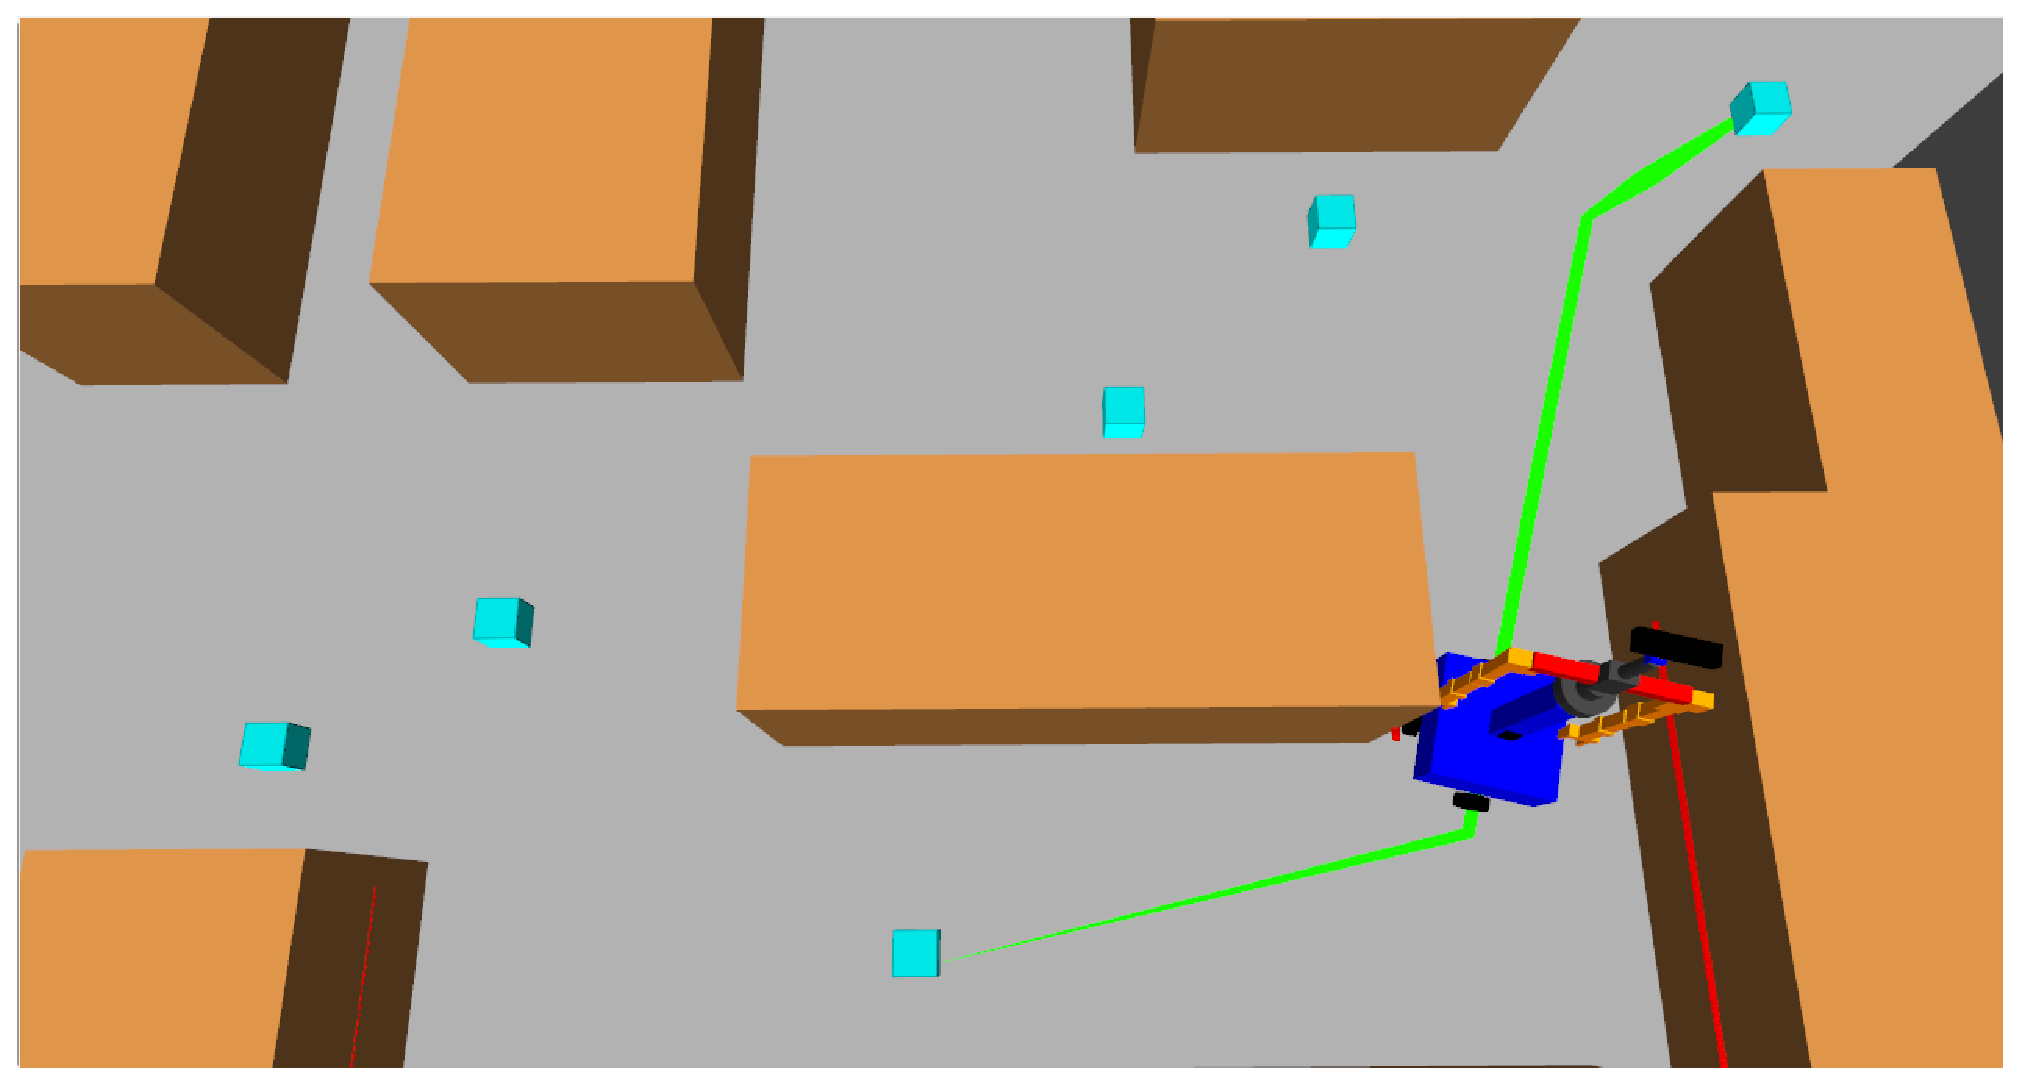
\includegraphics[width=\textwidth]{Figures/simulator1.eps} 
		%\caption{Path planning using an algorithm for a Topological Map.}
		%\label{fig:Simulator1}
	%%\end{subfigure}
	%%\begin{subfigure}{0.49\textwidth}
		%%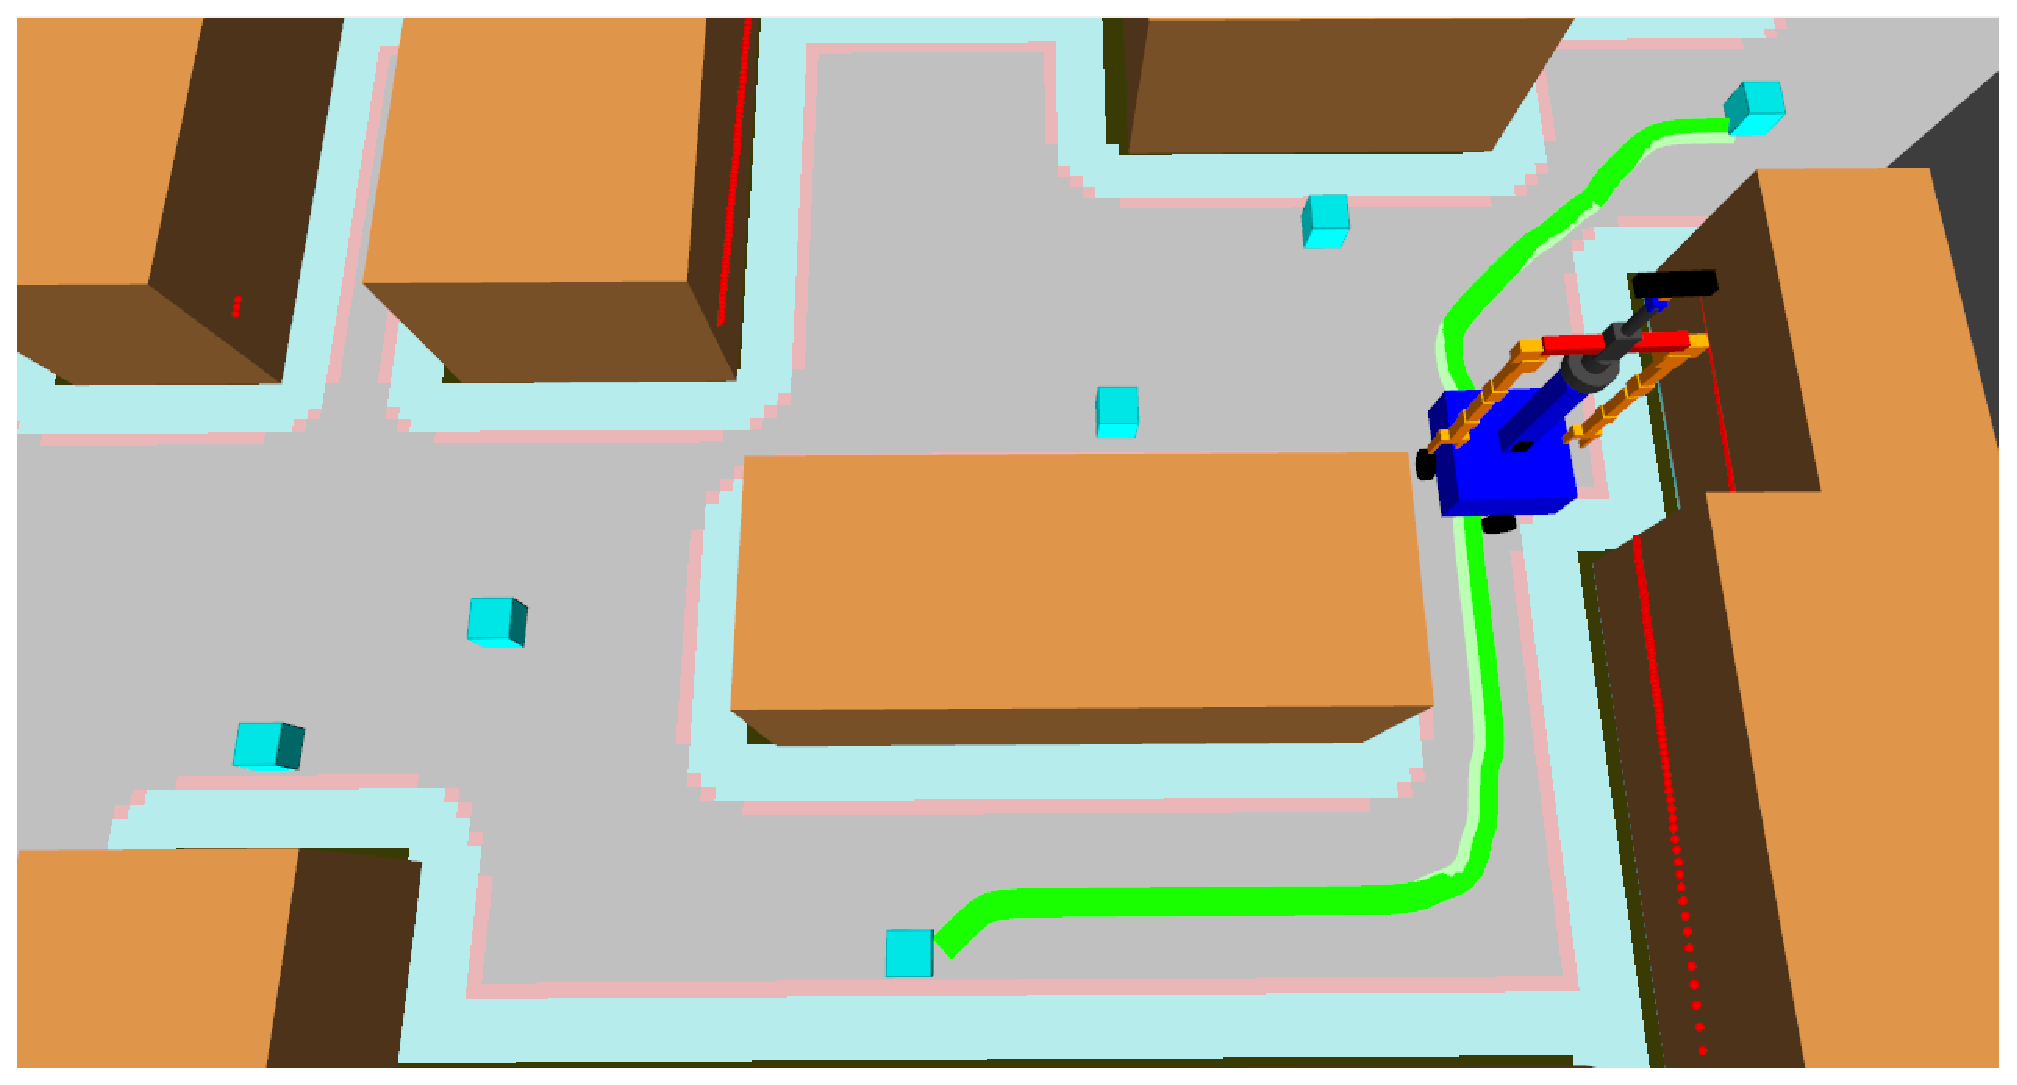
\includegraphics[width=\textwidth]{Figures/simulator2.eps}
		%%\caption{Path planning using an algorithm for an Occupancy Grid.}
		%%\label{fig:Simulator2}
		%%\end{subfigure}
	%%\caption{Test of a navigation algorithm using the graphical interface of the simulator. }
	%%\label{fig:Simulator}
%\end{figure}

%Figure \ref{fig:Simulator1} shows the robot simulated, the virtual representation of our laboratory and a path created using Dijkstra Algorithm based on a topological representation of the environment. 
%In contrast, Figure \ref{fig:Simulator2} shows a path created using the same robot and virtual environment, but using an 
%Occupancy Grid instead for representing the map.

%Thanks to the integration with ROS, after a simulation has been run, it allow us to test and visualise, in real time, the algorithms 
%in robot Justina for result analysis and comparison. Different algorithms in a wide-range of environment configurations has been 
%modelled and tested, both in simulation and in the real robot. 

\subsection{Action planning using space state representation}\label{subsec:ActionPln}
VIRBOT's task planning uses concepts from space-state search planning and hierarchical task networks,
as the ones used in classical STRIPS-like planners.

The plan is generated by an inference engine, CLIPS, that it uses a set of rules that represent a hierarchical structure of tasks.
The planning rules are useful for considering different situations, present in the environment, so that the robot can act accordingly.
The mechanism to generate a new plan starts with a spoken command, the representation of it  triggers a set of rules that generate the plan.
The spoken commands representation is defined by performing a syntactical analysis and a semantic interpretation of them using a 
natural language technique called Conceptual Dependency \cite{Schank}.
The Robot is able to perform atomic operations like grasping an object, moving itself
from on place to another, finding humans, etc. Then the objective of action planning is to
find a sequence of this atomic operations to achieve the desired goal.

This research was evaluated under the General Purpose Service Robot (GPSR) test of the @Home category, and after generating 30
random commands of the set of commands of this test, the robot was able to accomplish, trough action planning, the required actions
contained in the solution of the plans, shown in table \ref{tab:action_planning}.  

\begin{table}
\centering
\begin{tabular}{|l|l|}
\hline
Type of actions & Percentage of success\\
\hline
$\qquad$Navigation & $\qquad$75\\
$\qquad$Object Recognition & $\qquad$59\\
$\qquad$Face Recognition & $\qquad$72\\
$\qquad$Object Handling & $\qquad$42\\
$\qquad$Answering questions & $\qquad$87\\
\hline
\end{tabular}
\caption{Action planning success}
\label{tab:action_planning}
\end{table}




%\begin{figure}[H]
	%\centering
	%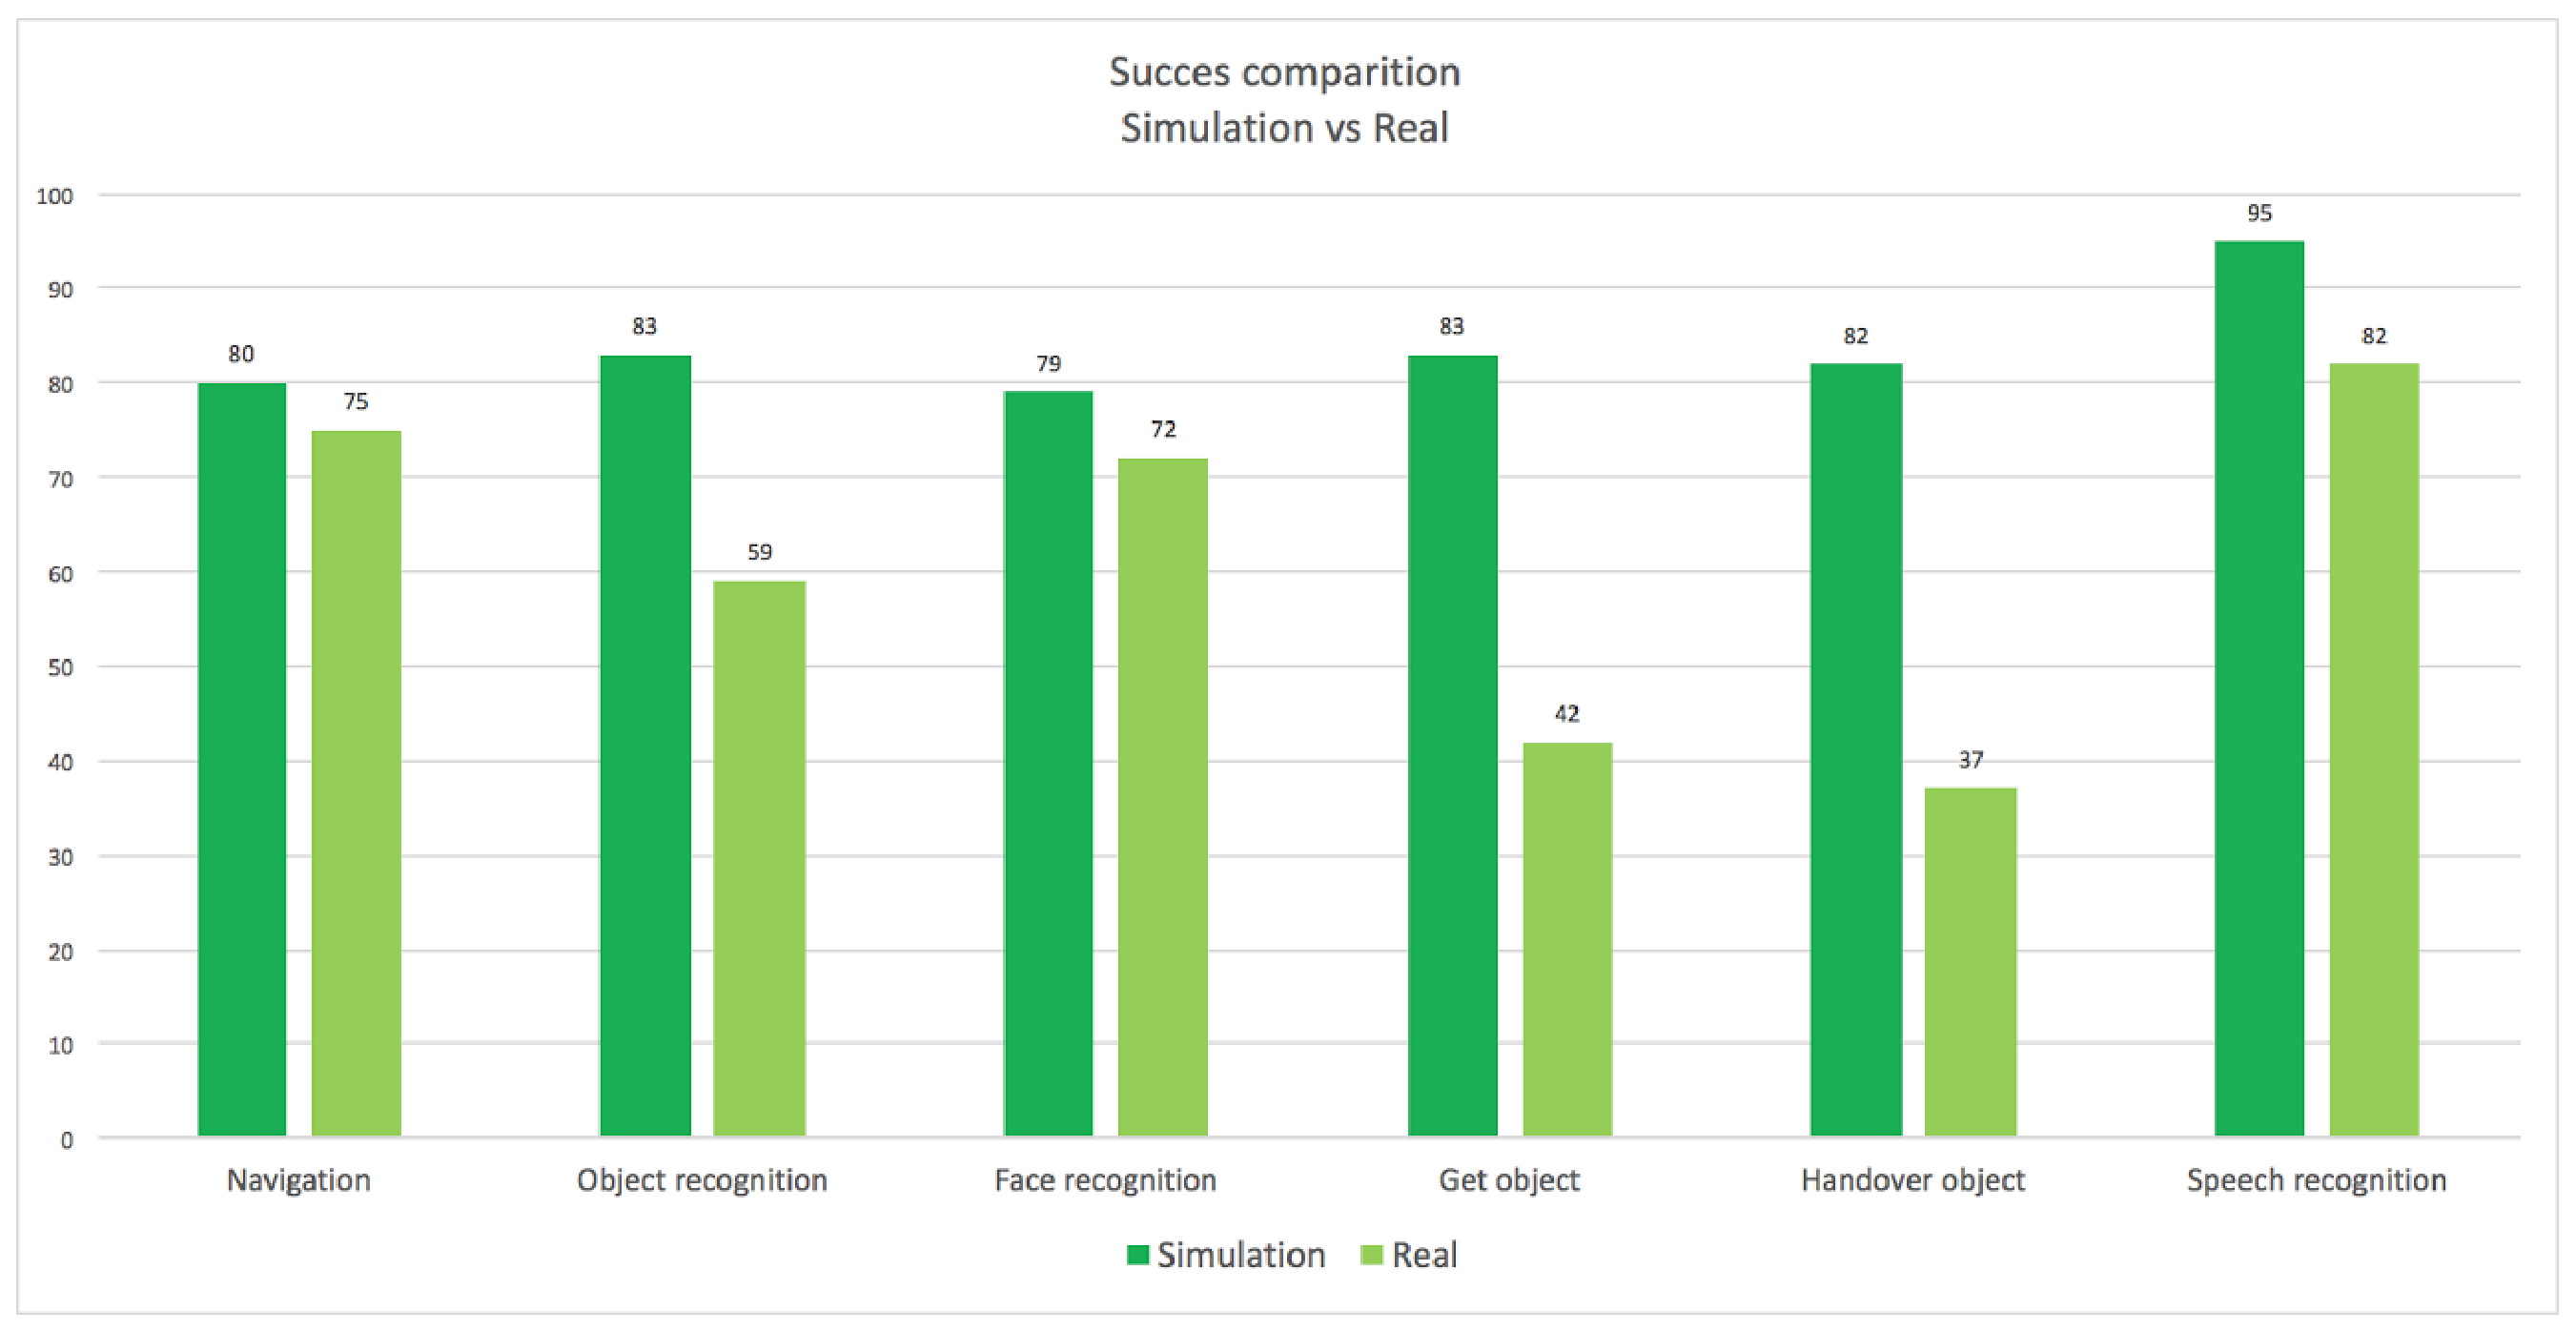
\includegraphics[width=0.8\textwidth]{Figures/taskPlanning.eps}
	%\caption{Comparison of success between simulated plans and real plans.}
	%\label{fig:taskPlanning}
%\end{figure}

%We have compared the number of successfully executed plans, both in simulation and with the real robot, as can be seen in Figure \ref{fig:taskPlanning}, for 100 executions for each action.

\subsection{Low or null texture objects recognition using RGB-D cameras}\label{subsec:objDet}

Currently, several robust techniques based on feature extraction and description exist for object recognition. However, if the objects 
are low textured, only a few number of features can be extracted, making the matching process unreliable. For these cases, 
we developed a method that combine three characteristics of the objects: color, size and shape, 
after a 3D detection and segmentation in a plane for each object.

Color information is extracted from the HSV space of the object's RGB pixels and it is represented by the histogram of the Hue 
components.
%but only for pixels with Saturation and Value above certain threshold. For pixels below these thresholds, two more bins are added to 
%the histogram. 
%For campaign histograms we used the histogram Intersection \cite{swain1991_HistoInter}.

The size and shape is estimated from the object's point cloud, which are obtained using an oriented bounding box (OBB) of the points
cloud.
% as follow: the base of the OBB is obtained from the oriented bounding rectangle of the projection of the points in the plane below 
%them. The heights are obtained from the maximum distance of the points to the plane. 
The shape is characterized using the Hu Moments \cite{hu1962_moments} of the convex hull calculated from the points projected over the
plane below them. 
Thus, with these representations an histogram is obtained for each of the objects and  
for the recognition process we compare the objects' histograms with the histogram of the object to be recognized.

%\begin{align*}
%H &= H_H \cup H_S \cup H_V \\
%H_H &=  B_1 \cup B_2 \cup ... \cup B_N \text{ donde } H=[0,255], V=[50,255], S=[50,255] \\
%H_S &=  B_{N+1} \text{ donde } H=[0,255], V=[0,50], S=[50,255] \\
%H_V &=  B_{N+2} \text{ donde } H=[0,255], V=[50,255], S=[0,50]
%\end{align*}

%, removing candidates below a certain threshold for each step. At the end, from the remaining candidates, we select the best one according to a color-based similarity function. 


%Por tanto esto queda como:

%\begin{equation}
%H = \underbrace{ B_1 \cup B_2 \cup ... \cup B_N }_{H=[0,255], V=[50,255], S=[50,255]} \cup \underbrace{B_{N+1}}_{H=[0,255], V=[0,50], S=[50,255]} \cup \underbrace{B_{N+2}}_{H=[0,255], V=[50,255], S=[0,50]} 
%\end{equation}


 The histograms are compared using histogram intersections, \cite{swain1991_HistoInter}:

\begin{equation}
H(I,M) = \frac{ \sum_{j=1}^{n} \min(I_j, M_j) }{ \sum_{j=1}^{n} M_j }
\end{equation}

Where \(I\) is the histogram of the object to be recognized, \(M\) represents one of the stored objects' histograms and \(n\) is the
number of bins in the histograms. 

This method has been tested experimentally, showing fast and robust results for changes in light, scale, and rotation in a plane
parallel to the plane below the object. 
Figure \ref{fig:objReco} shows an example of objects' recognition on a shelf (multiple planes).

\begin{figure}
	\centering
	\begin{subfigure}{0.49\textwidth}
		%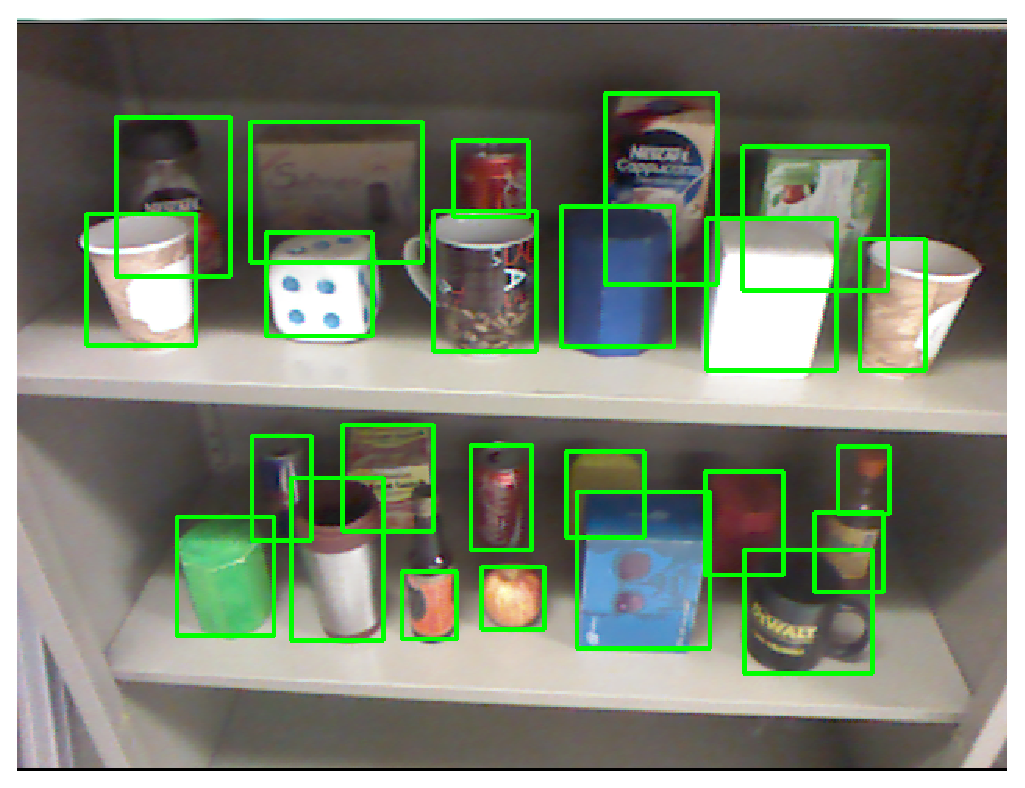
\includegraphics[width=\textwidth]{Figures/objetos1.eps}
		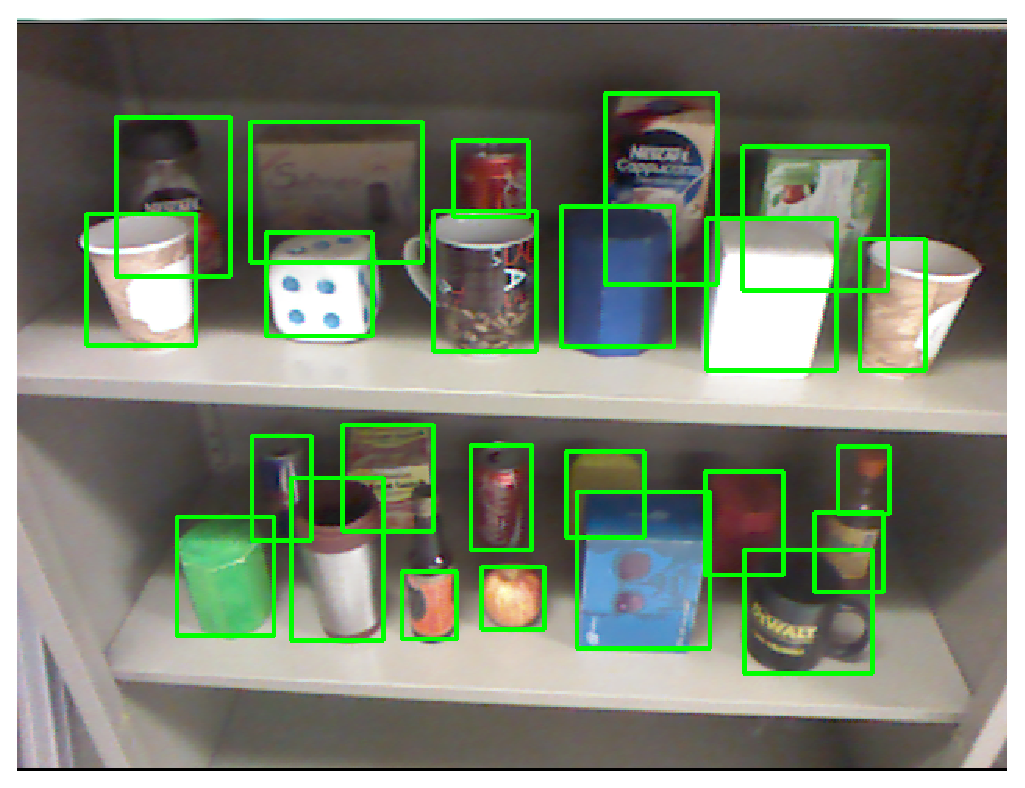
\includegraphics[angle=0, height=3cm, width=4cm]{Figures/objetos1.eps}
		\caption{Objects can be segmented even with occlusions.}
		\label{fig:objReco2}
	\end{subfigure}
	\begin{subfigure}{0.49\textwidth}
		%
\includegraphics[width=\textwidth]{Figures/objetos2.eps} 
		
\includegraphics[angle=0, height=3cm, width=4cm]{Figures/objetos2.eps} 
		\caption{ Point clouds corresponding to each segmented object.}
		\label{fig:objReco1}
	\end{subfigure}
	\caption{Example of object segmentation on several planes.}
	\label{fig:objReco}
\end{figure}

Table \ref{tab:comp} shows the results obtained by comparing this histogram method with a SIFT algorithm for 25 objects
without or almost no texture.


\begin{table}
\centering
\begin{tabular}{|c||c|c|c|c|}
 \hline
%System & \% Recognized & \% No recognized & \% Errors & $\tau_{avg}$ \\
System & \% Recognized & \% No recognized  \\
 \hline
Proposed & \textbf{91.333} & \textbf{7.666} \\
SIFT & 22.333 & 77.666 \\
\hline
\end{tabular}
\\
\caption{Comparison of recognition of objects using color, size and shape histograms and SIFT.}
\label{tab:comp}
\end{table}

As we can see for the results on table \ref{tab:comp} this technique outperforms the SIFT one.



%%%%%%%%%%%%%%%%%%%%%%%%%%
%%%  CONCLUSION AND FUTURE WORK  %%%
%%%%%%%%%%%%%%%%%%%%%%%%%%

\section{Conclusions and future work}\label{sec:conclusions}
It is clear, that during the 11 years in which our team Pumas has been participated in the RoboCup and 2 years
in the Rockin \cite{Rockin} in the category @Home, the performance and research developed, in the service robot area, in our 
laboratory has been improved considerably.
Our service robot architecture, the VIRBOT, has been evolving according to the requirement that these robotics
competitions asked each year.
In these years, the full system has been improved, both in hardware and software, having reliable performance and showing promising 
results. Particularly, this year, we have a new omnidirectional mobile base for navigation and a new torso. 
In terms of software, we have change the way of conceiving the tests of the competition: from static state machines to inferred
action planning generated by a rule based system. 
As for future work, the computer vision algorithms will be improved by using Hidden Markov Models (HMM) to have a better 
recognition of objects and persons. Also, it will be explored fault tolerant systems to help the robot to recover from failures.
We consider that if our team becomes a parnert in the Joint Research for the standar Toyota Human Support Robot 
platform, the majority of our software, developed so far, can be used directly in this platform and our robotics 
research can be improved sustanciably.

 


%\bibliographystyle{unsrt}
%\bibliography{References}
\bibliographystyle{unsrt}
\bibliography{bibliography,justina}

\begin{thebibliography}{1}

%\bibitem{Robocup}
%{\em RoboCup@Home} 2015: Rule and Regulations, Loy van Beek, Mauricio
%Matamoros and  Sven Wachsmuth,
%http://www.robocupathome.org/rules/2015\_rulebook.pdf, 2015.

\bibitem{virbot}
{\em ViRbot: A System for the Operation of Mobile Robots}, Savage, Jesus and et al, RoboCup 2007: Robot Soccer World Cup XI,
pp 512-519, Springer Berlin Heidelberg, 2007.

\bibitem{muller}
{\em The Design of Intelligent Agents: A Layered Approach}, Muller, Jorg P,Springer-Verlag New York, Inc.1997.


\bibitem{Marco}
{\em Parallel implementation of roadmap construction for mobile robots using rgb-d cameras},
Marco Negrete, Jes{\'u}s Savage, Jes{\'u}s Cruz, and Jaime M{\'a}rquez, OGRW2014, pages 184--187, 2014.

\bibitem{Schank}
{\em Conceptual dependency and its descendants}, Steven L. Lytinen, Computers \& Mathematics with Applications, 1992.

\bibitem{hu1962_moments}
{\em Visual pattern recognition by moment invariants}, Ming-Kuei Hu, IRE Transactions on Information Theory, 8(2):179--187, 1962.

\bibitem{swain1991_HistoInter}
{\em Color indexing},  Michael~J Swain and Dana~H Ballard, International journal of computer vision, 7(1):11--32, 1991.


\bibitem{Rockin}
http://rockinrobotchallenge.eu/home.php


\end{thebibliography}





\end{document} 

%%% Local Variables:
%%% mode: latex
%%% TeX-master: t
%%% End:
